%%%%%%%%%%%%%%%%%%%%%%%%%%%%%%%%%%%%%%%%%%%%%%%%%%%%%%%%%%%%%%%%%%%%%%%%%%%%%%%%
%neutrino_physics.tex: Chapter on Long Lived Neutral Particle physics:
%%%%%%%%%%%%%%%%%%%%%%%%%%%%%%%%%%%%%%%%%%%%%%%%%%%%%%%%%%%%%%%%%%%%%%%%%%%%%%%%

% Science Chapter: What is Long-Lived Physics particles?
\chapter{Phenomenology of Long-Lived Particles}
\label{Long_Lived_Particle_physics_chapter}
%\ref{Physics}


\section{The Standard Model of Particle Physics}
%%%%%%%%%%%%%%%%%%%%%%%%%%%%%%%%%%%%%%%
The Standard Model~(SM) of particle physics provides a thorough and experimentally verified mathematical model description of the fundamental constituents of visible matter and its interactions~(except gravity) in the universe. Predictions of particle properties and interactions by the SM agree with most of the available experimental data with unmatched precision.
\newline
Despite the numerous success of the SM, there are some theoretical and experimental inconsistencies with the SM such as the observation of Dark Matter~(DM) in the universe which is indescribable by the SM, the observation of neutrino oscillation and neutrino masses unexplained by the SM and the absence of gravitational interactions in the SM. These shortcomings of the SM, promotes the believe that the SM is part of a more general model. A candidate mathematical model beyond the SM which provides possible explanations for the above observations is \textit{supersymmetery}.
\newline
In the next sections, we briefly describe the major components of the SM, its strengths and limitations and also introduce supersymmetry as a leading candidate for models beyond the SM.
\subsection{Main Components of the SM}
Mass, charge, spin and lifetime can be used to identify and categorize fundamental particles of nature.
Partices with the same charge, mass and spin but opposite charge are called \textit{Anti-particles} while particles with equal amounts for positive and negative charge are said to be neutral. A interesting classification of particles and anti-particles is using their \textit{spin}~($s$).
A particle's spin is an \textit{internal quantum number} expressed as $n\hbar$, where $n$ can be \textit{integer} or \textit{half-integer}.
Half-integer spin~($\frac{1}{2},\frac{3}{2},\cdots \times\hbar$) particles obey a \textit{Fermi-Dirac} distribution or statistics and are called \textit{fermions}. Integer spin particles~($0,1,2,\cdots\times \hbar$) obey \textit{Bose-Einstein} statistics and are called \textit{Bosons}. 
No two identical fermions can occupy the same quantum state but any number of bosons can occupy a given quantum state.
\newline
Fermions are the fundamental building blocks of matter while bosons mediate interactions between fermions. No particle with spin, $s=0\hbar$, had ever been experimentally observed until the 4th of July 2012 when the \textit{Higgs} boson with spin, $s = 0\hbar$, was observed\cite{HIGGSD}. The Higgs boson is responsible for providing mass to both fermions and bosons. Its discovery completes the SM. 

The particle spin set, $S$, shown in Equation \ref{eq:SPIN}, shows the spins of particles discovered and yet-to-be-discovered in the universe.
\begin{equation*}{\label{eq:SPIN}}
S =\left \{s=\Big(\cdots \mathbf{0}, \frac{1}{2}, 1,  \frac{3}{2}, 2  \cdots \Big).\hbar\right \}
\end{equation*}
%where  $s$ is the spin of a particle and $\hbar$ is the \textit{Planck} constant. 
Looking at the set $S$, our present and possibly future understanding of particles in the universe can  be summarize as follows:
 \begin{itemize}
  \item $\mathbf{S = \frac{1}{2}\hbar}$ Particles which make up visible matter in the universe.
  \item $\mathbf{S = 1\hbar}$ Particles mediating gauge interactions.
  \item $\mathbf{S = 0\hbar}$ Particle responsible for giving mass to other particles.
  \item $\mathbf{S = 2\hbar}$ Yet-to-be-discovered particle mediating  gravitational interactions.
  \item $\mathbf{S = \frac{3}{2}\hbar}$ Yet-to-be-discovered particle likely to make up \textcolor{red}{\textbf{Dark Matter}?}
 \end{itemize}
It is interesting to note that the set particles with spins, $s =\Big\{\mathbf{0}, \frac{1}{2}, 1\Big\}\hbar$, describes precisely only $4.6$\% of the entire matter in the universe through the SM. 
%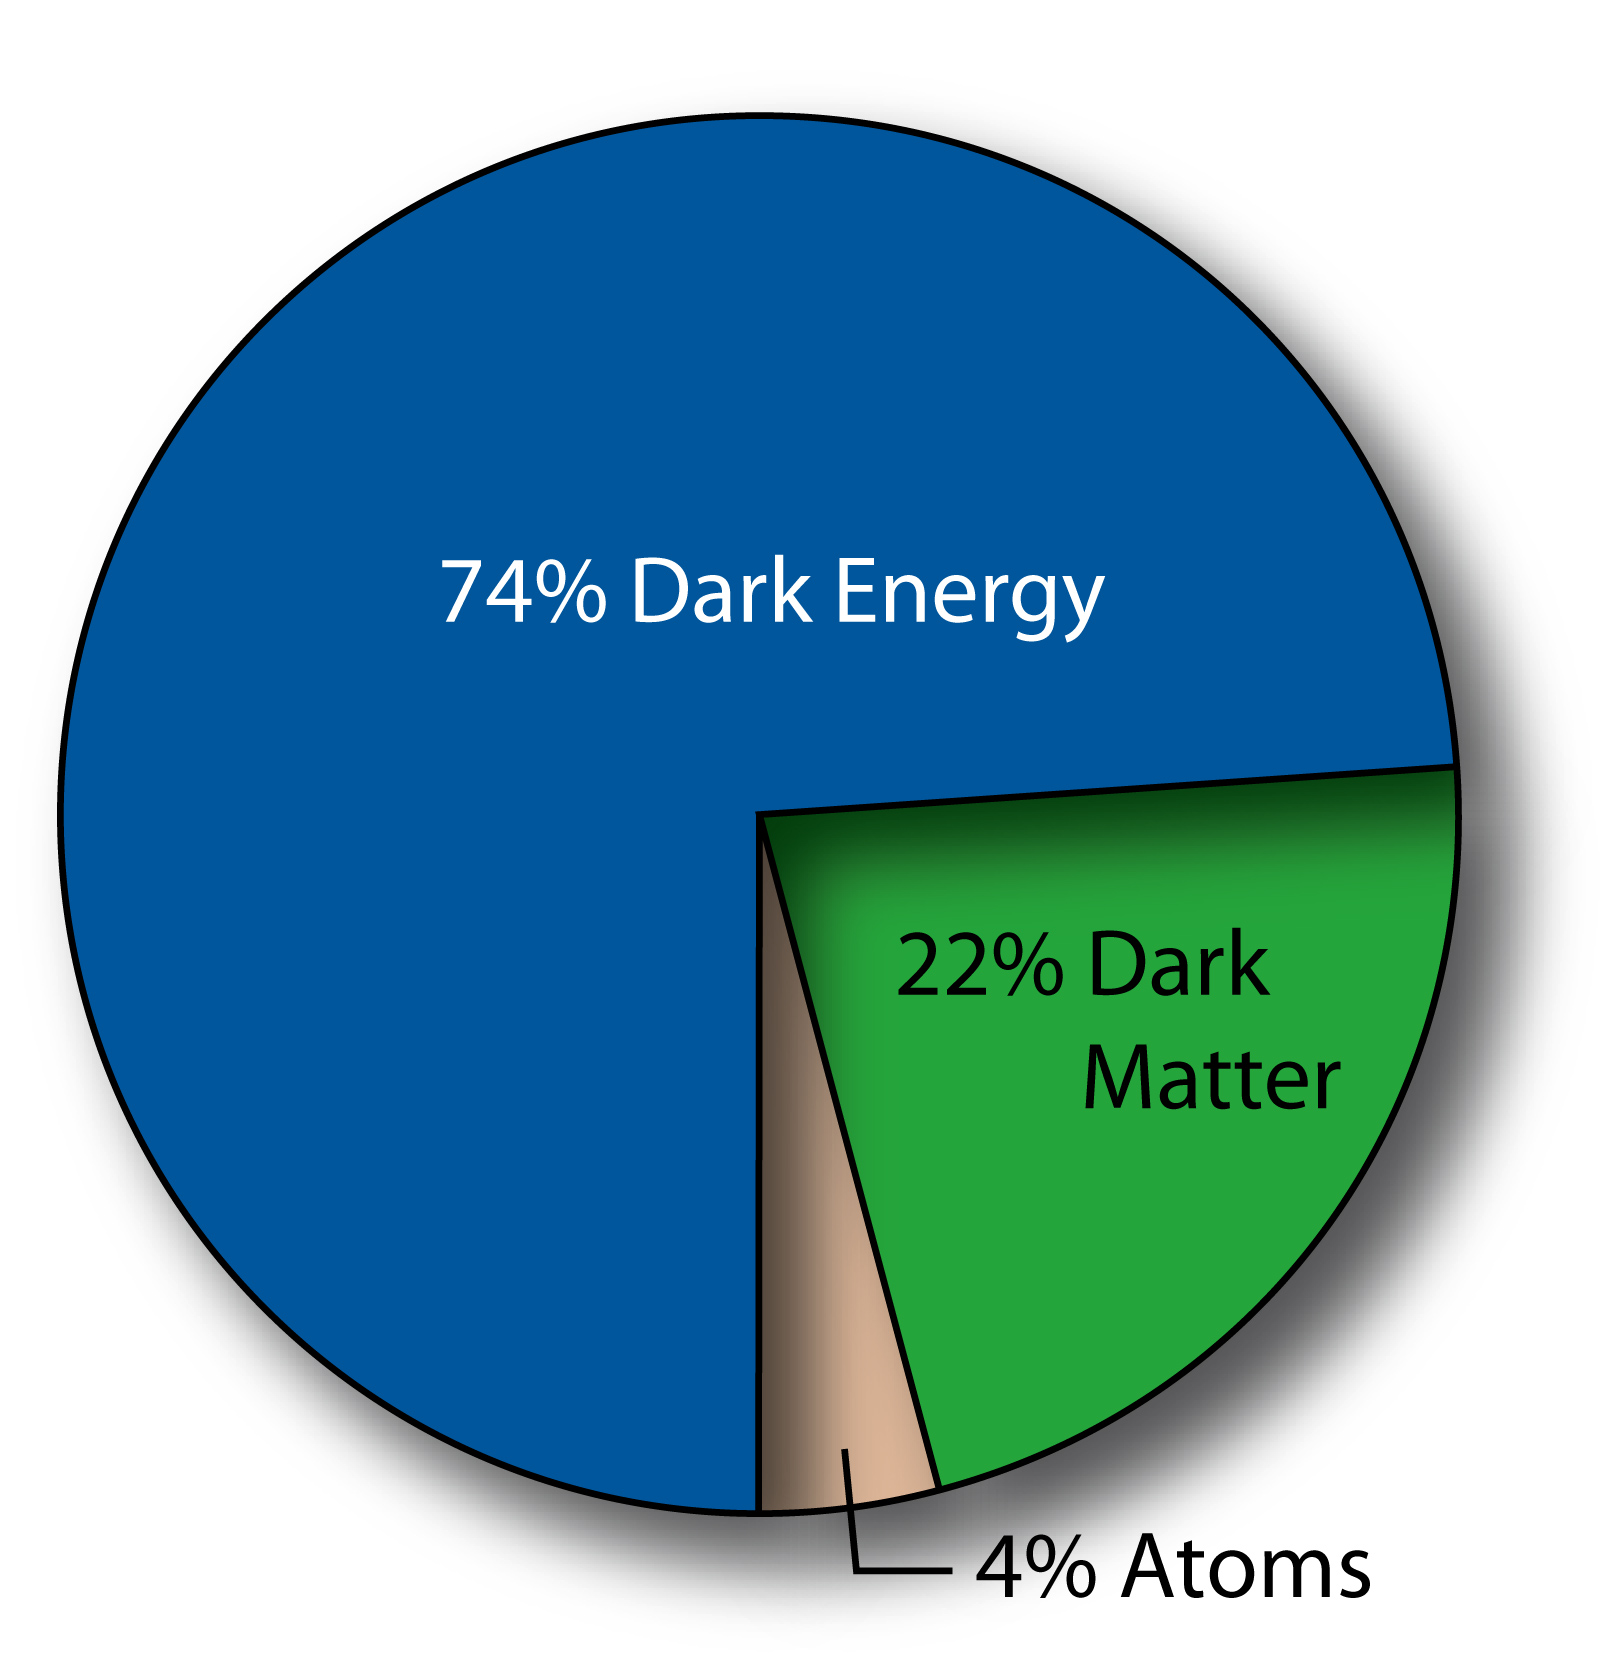
\includegraphics[height=1.7cm,width=0.25\paperwidth]{THESISPLOTS/UniversePie30.jpg}
%\end{frame}
%The above particles and their nature of interaction is described mathematically using the 
The SM is a \textit{relativistic quantum field theory} in which particles are represented as \textit{quantum fields} and their dynamics and interaction with other particles is expressed using a mathematical functions called \textit{Lagrangian density}, $\mathcal{L}$. The Lagrangian density is invariant under certain transformations or symmetries and carries the description of the dynamics of fermions, bosons and their interactions with the Higgs boson. Fermions and bosons obtain their mass by interacting with the Higgs boson through a process crucial to the SM called \textit{Higgs Mechanism}.
Our brief description of the SM, will be divided into the following sections:
\begin{itemize}
\item \textbf{\textit{Fermions}}: All of visible matter is described using fermion fields.
\item \textbf{\textit{Interactions}}: Fermions interact either through electromagnetic, weak and strong interactions with vector bosons mediating  the interactions. An interaction is the realization of some generic symmetry and associated with this symmetry is a conserved quantity.
\item \textbf{\textit{Spontaneous Symmetry Breaking or Higgs Mechanism}}: Fermions originally have no mass. They get their mass by interacting with the Higgs field through the \textit{Higgs mechanism}. New states of matter or fermions can be formed through mixing with other states of matter or fermions.

\end{itemize}
\subsection*{Fermions}
The \textit{Dirac} equation given by Equation \ref{eq:DIRAC} is part of the SM Lagrangian describing
\begin{equation}{\label{eq:DIRAC}}
\mathcal{L}(\bar{\Ppsi},\Ppsi, G^{\mu}) = \bar{\Ppsi}\left(i \Pphoton^{\mu}\mathcal{D}_{\mu} - m \right)\Ppsi. 
\end{equation}
fermion dynamics with its electromagnetic interaction through the $\mathcal{D}_{\mu}$ term. 
In the full SM Lagrangian, including the description of electromagnetic, weak and strong interactions, fermions participate in these interactions as pairs or \textit{doublets} called a representation. According to the SM, fermions exists as either leptons~($\Plepton$) or quarks~($\Pquark $) and come in $3$ \textit{generations}. The SM provides no explanation for the existence of only 3 generations.
Leptons can participate in electromagnetic and weak interactions but not in strong interactions while quarks can participate in both interactions and strong interactions. Leptons have integer charge while quarks have fractional charge. The $3$ generations of quarks and leptons also known as \textit{flavors} are arranged in a mass hierarchy with the third generation being the heaviest. The second and third generations are meta stable can disintegrate or \textit{decay} into the first generation through weak interactions. 
A lepton pair consists of a particular lepton flavor and its corresponding neutral neutrino type. There is a corresponding neutrino for each lepton generation. For example, an \texttt{electron}~($\Pe$) and its corresponding electron \texttt{neutrino}~($\Pnue$) make the first generation pair,($\Pe,\Pnue$ ). Other lepton flavors include \texttt{muon}~($\Pmu$) and \texttt{muon neutrino}~($ \Pnum$) pair~($\Pmu,\Pnum $) and \texttt{tau}~($\Ptau$) and \texttt{tau neutrino}~($\Pnut$) pair~($\Ptau,\Pnut$ ).
In the SM, neutrinos are described as having no mass, however, numerous experiments have confirmed that neutrinos have a very tiny mass~(order of electronvolts~(eV)) and can oscillate from one generation into another over sufficiently large distances.
\newline
For quarks, a first generation pair of quarks consists of an "\textit{up-type}" and a "\textit{down-type}" quark. In addition to the electric charge, quarks also carry a \textit{color} charge and as a result can equally participate in strong interactions. \textit{Up-type} quarks like \texttt{up}~($\Pup$), \texttt{charm}~($\Pcharm$), \texttt{top}~($\Ptop$) have charge of $+\frac{2}{3}$ and \textit{down-type} quarks such as \texttt{down}~($\Pdown$), \texttt{strange}~($\Pstrange$), \texttt{bottom}~($\Pbottom$) have a charge of $-\frac{1}{3}$. Charges are expressed in units of elementary charge e. The quark include ($\Pup, \Pdown$) is the first generation  and ($\Pcharm, \Pstrange$) and ($\Ptop, \Pbottom $) are respectively, the second and third generations. Quarks do not exist as free particles in nature but are found bound forming composite particles like \textit{pions} and \textit{protons} collectively called \textit{hadrons}. Hadrons consisting of a quark and antiquark~(same mass and spin as a quark but different charge) bound together are called \textit{mesons},\eg pions~(\Ppizero,\Ppipm), while those with at least 3 quarks bound together are called \textit{baryons}, \eg protons.  The distributions of these quarks inside hadrons can be modeled using  \textit{parton distribution functions}~(PDF) which depends on the fraction of momentum of the given hadron carried by each quark.
\newline
One can distinguish between "\texttt{Left}" from the  "\texttt{Right}" handed quarks and leptons from the nature of their interaction with electroweak bosons.
\paragraph*{}  
Since most particles in the second and third generation are meta-stable, and do decay into the first generation particles, it is possible to describe all visible matter in our universe using only one generation of leptons, \texttt{electron} and the \texttt{electron neutrino}~($\Pe$,$\Pnu$) and one generation of quarks, \texttt{up-quark} and \texttt{down quark}~($\Pup$,$\Pdown$). 
 
\subsection*{Interactions}
Interaction between fermions is mediated by vector \textit{bosons} with spin, $s=1\hbar$. The SM describes the electromagnetic, weak and strong force and their force mediators. The \textit{electromagnetic force} whose force carrier is a massless vector boson; the \textit{photon}~($\Pphoton$), is described using the mathematical formulation called \textit{Quantum Electrodynamics}~(QED). It is responsible for the interaction of light with matter. The \textit{weak force} has 3 massive vector bosons; $\PWmp$, $\PZzero$, as its force mediators and it is responsible for the decay of the second and third generation quarks into the first generation. The weak force was independently developed by Sidney Glashow, Abdus Salam and Steven Weinberg \cite{SWG} in the 1960s unifying it with the electromagnetic force in a mathematical formulation called the \textit{Electro-Weak Field Theory}. The 3 massive vector bosons were predicted in the late 1960s and were eventually discovered at CERN in 1983. Finally, the \textit{strong force} described using the mathematical formulation of \textit{Quantum Chromodynamics}~(QCD) has a massless \textit{gluons}~($\Pgluon$) as its force mediators. The strong force like the weak force is a nuclear force, however, the same unification  of the weak and electromagnetic forces is not observed with the strong force. It remains an open question whether at much higher energies, all 3 forces become unified behaving as a single force. \newline
It is speculated that the gravity interaction not described by the SM, is mediated by a spin-2 particle called the \textit{graviton} which is yet to be discovered.
%The table below show some the property of the force mediating particles in SM.

%\begin{equation}
% "PLEASE INSERT TABLE/DIAGRAM FOR GAUGE BOSONS HERE!"
%\end{equation}

%The current frame work of the SM was formulated with inputs from theory and results from several experiments so it in not uncommon to introduce mathematical concepts and constructs to describe the SM in an elegant manner. It is with this spirit that we will continue the rest of this section.

  The formulation of the SM, relies on the concept of \textit{symmetry} and \textit{conserved quantum numbers}. A symmetry is a transformation which leaves invariant the dynamics~(Lagrangian density, $\mathcal{L}$) describing a particle interaction. Every particle interaction is associated with a symmetry and a conserved quantity. The conserved quantity  is called \textit{conserved quantum number}. Belonging to the SM, are \textit{gauge symmetries}, meaning the SM Lagrangian remains invariant under  space-time dependent gauge transformations.
The gauge symmetry of the SM is a combination of 3 different gauge symmetries; $SU(3)_{C}$, $SU(2)_{L}$ and $U(1)_{Y}$, each describing a particular particle interaction type. This combination is expressed  as given in equation \ref{eq:SYM}.

\begin{equation}{\label{eq:SYM}}
SU(3)_{C} \otimes SU(2)_{L} \otimes U(1)_{Y}
\end{equation}

%The symmetry groups describe the following parts of the SM interactions:
 %defines the strong nuclear interaction where quarks with color charge C are coupled to massless  eight( octet ) gluons in the frame work of QCD. The surprising phenomenon here is that unlike electromagnetic interactions ~(QED) where massless photons cannot interact with each other, these massless guons can interact with each since they carry color charge. There are three color charges.
\paragraph*{}
$SU(3)_{C}$ is the gauge symmetry associated with strong interactions and the conserved quantum number is the \textit{color}~($C$) charge allowing the gluon to interact with itself and with quarks. There are $8$~(in the \textit{octet} representation of the $SU(3)$ gauge symmetry) colorless and massless gluons and three different color type quarks for each quark flavor. Anti-quarks carry anti-color charges. Leptons, like electrons, do not carry the color charge and as a result cannot participate in strong interactions.
%As previously mentioned, no free quark has been observed, rather, quarks exist in nature in the form of bound states called \textit{hadrons}. Hadrons can either be \textit{mesons}, which means, they are made up of a quark-antiquark pair like pions~(\Ppizero,\Ppipm) or \textit{baryons}, which means they are made up of 3 quarks like protons. Recent experiments have observe bound states consisting of $4$ quarks \cite{Quarks}, which remain consistent with the nature of  strong interactions between quarks in nuclei.
\paragraph*{}
 $SU(2)_{L} \otimes U(1)_{Y}$ is the gauge transformation group with conserved quantum number, \textit{isospin}~($T_{3}$), necessary for the electroweak interaction. Corresponding to the $SU(2)\otimes U(1)$ gauge group, there are $4$ massless gauge bosons, $W^{1,2,3}_{\mu}, B_{\mu} $, which combine to form the physical electroweak bosons of charged $\PWmp$ and neutral $\PZzero$ and $\Pphoton$. 
The $\PWmp$ and $\PZzero$, through the spontaneous breaking of the electro-weak symmetry, obtain their masses. These physical mass states is responsible for quarks to be able to transform from one generation to the other. These bosons couple using the "charge" of the weak interaction called \textit{isospin}, $T_{3}$, and the \textit{hypercharge}, $Y$, to matter fields. The $\PWmp$ only interacts with \texttt{left-handed} fermions and \texttt{right-handed} anti-fermions. This leads to a phenomenon called \textit{parity} violation. The electromagnetic charge, $Q$, is the result of a combination of the third component of the weak isospin, $T_{3}$ and the hyper charge, $Y$, through the following relation:
\begin{equation}
Q = T_{3} + \frac{Y}{2}
\end{equation}

Left handed fermions have $T_{3} = \pm \frac{1}{2}$ and form representations known as isospin \textit{doublets},  while, right-handed fermions have $T_{3} = 0$ and form isospin \textit{singlets}  in the SM . 
The particles in the SM together in their representations given by the gauge symmetry as \textit{multiplets(doublets, triplets}, etc) and the corresponding conserved quantum numbers is presented in Table \ref{tab:SM}.
The $SU(2)_{L} \otimes U(1)_{Y}$ guage group is a combination of two symmetry groups with coupling strengths $g$ and $g^{\prime}$ connected to the electric charge of each fermion as $e = g\sin \theta_{w} = g^{\prime}\cos \theta_{w}$.


 The angle, $\theta_{w}$, is the \textit{Weinberg angle}, $sin^{2}\theta_{w} \approx 0.231$ is not predicted by the SM but measured from experiments.
Gauge bosons can rotate from their \textit{weak} eigen states to physically observed states using this angle.
%The physically observed gauge bosons are a rotation of the weak eigenstates involving the Weinberg angle given as:
\begin{equation}
 \PWmp_{\mu} = \frac{W^{1}_{\mu} \mp i W^{2}_{\mu}}{\sqrt{2}}, \quad \quad 
 {\begin{pmatrix} A_{\mu} \\ Z_{\mu}  \end{pmatrix} } = {\begin{pmatrix}  \cos{\theta_{w}} & \sin{\theta_{w}} \\ -\sin{\theta_{w}} & \cos{\theta_{w}}   \end{pmatrix}}  {\begin{pmatrix} B_{\mu} \\ W^{3}_{\mu} \end{pmatrix} }
\end{equation}
This angle,$\theta_{w}$, also allows for the transformation of a quark from one flavor into another through the $\PWmp$ bosons. In the lepton sector, according to formulation of the SM, such flavor transformation could in principle be possible but does not lead to any possible observable effects as nuetrinos are considered to be massless in the SM. On the other hand, recent neutrino experiments have proven otherwise, as mixing between different neutrino types have been observed, indicating that neutrinos are not massless as thought but rather do have mass. The transformation of quarks into different flavors is a typical interaction happening inside the core of our sun in the decay of neutrons to protons and similarly in a nuclear reactor. The complete transformation of all quark flavors is described by the \textit{Cabibbo-Kobayashi-Maskawa}~(CKM) 3 by 3 matrix whose elements are parameters only measured from experiments and not predicted by the SM.
%This angle participates in an important phenomenon in SM known as quark mixing. Unfortunately in the current simplest state of SM, there are no lepton mixing(due to a global symmetry called lepton number conservation) even though the recent discovery of neutrino masses existence \cite{} hints at the possibility of such a mixing in the lepton flavour sector.
%Nevertheless, in the quark sector, it is possible for the $W^{\pm}$ to change the flavour of a given quark, for example and up-type quark u can transition to a down-type quark d. This type of transitions are referred to as Flavour Changing Charge Currents~(FCCC). However, it is not possible for $Z^{0}$ to change the flavour of a quark but also lead to small violation of parity. There is active research to discover large Flavour Changing Neutral Currents~(FCNC) from certain  weak interactions since most of these are suppressed.
%The quark mixing is entirely described using a 3 by 3 component matrix known as the Cabibbo-Kobayashi-Maskawa ~(CKM) matrix given in equation below:

%\begin{equation}
%The CKM matrix
%\end{equation}
%The entire components of this matrix is measured from experiment and not derived from the SM.
\clearpage
\begin{center}
\centering
\bfseries{Particle and Their Gauge Symmetry Representation}
\begin{tabular}{c|c|c|c}
 \toprule
\bfseries{Particle Name(Symbol)} & \bfseries{Spin} & \bfseries{Multiplet} & \bfseries {$SU(3)_{C} \otimes SU(2)_{L} \otimes U(1)_{Y}$}\\
\hline\hline
 Quarks ($Q$) & 1/2 & $(\Pup_{L}, \Pdown_{L})$  & $(\mathbf{3}, \mathbf{2}, \frac{1}{6})$\\
 $\bar{\Pup}$ & 1/2 & ${\Pup^{\dagger}_{R}} $& $(\mathbf{\bar{3}}, \mathbf{1}, -\frac{2}{3})$\\
 $\bar{\Pdown}$ & 1/2 & ${\Pdown^{\dagger}_{R}} $& $(\mathbf{\bar{3}}, \mathbf{1}, \frac{1}{3})$\\
 ($\times 3$ families) & & & \\
\hline
 Leptons($L$) & 1/2 &  $(\Pnu, \Pe_{L} )$ & $(\mathbf{1}, \mathbf{2}, -\frac{1}{2})$\\
 $\bar{\Pe}$ & 1/2 & ${\Pe^{\dagger}_{R}} $& $(\mathbf{\bar{1}}, \mathbf{1}, 1)$\\
 ($\times 3$ families) & & & \\
 & 1/2 & $\Pneutrino^{\dagger}_{R}$ & $(\mathbf{\bar{1}}, \mathbf{1}, 1)$ \\
\hline
Higgs ($\PHiggs_{u} $) & 0 & $(\PSHiggsplus_{u}, \PSHiggszero_{u})$ &  $(\mathbf{1}, \mathbf{2}, +\frac{1}{2})$ \\
Higgs($\PHiggs_{d}$)   & 0 & $(\PSHiggsplus_{d}, \PSHiggsminus_{d})$ &  $(\mathbf{1}, \mathbf{2}, -\frac{1}{2})$ \\
\hline\hline
\bfseries{Force Carriers} &  & & \\
 Gluons & 1 & $\Pgluon$ & $(\mathbf{8}, \mathbf{1}, 0)$ \\
 (Strong Force) & & & \\
 \hline
 $\PW$ bosons & 1 & $\PW$ & $(\mathbf{1}, \mathbf{3}, 0)$ \\
 $\PB$ boson & 1 & $\PBzero$ & $(\mathbf{1}, \mathbf{1}, 0)$ \\
 (Electro-Weak Force) & & & \\
\hline 
 \bottomrule
\end{tabular}
\captionof{table}{SM particles and their gauge multiplets(representation) with quantum numbers.
the numbers for example $(\mathbf{3}, \mathbf{2}, \frac{1}{6})$ means (\textit{triplet},\textit{doublet}, $Y = 1/6$) representations. }
\label{tab:SM} 
\end{center}

%\subsection*{Quantum Chromodynamics and Parton Distribution Functions}
%\paragraph*{}
%The strong nuclear interactions described by QCD is based on the $SU(3)_{C}$ gauge group. Only quarks and gluons are involved in this interaction. Each quark can exists in three different strong "charge" called \textit{color} ( dubbed are red, green and blue ) thus forming a color triplet. Anti-quarks also carry opposite color charges. The color strength is the same for all three colors. Gluons unlike photons carry a combination of color and anti-color charge which lead to the self interaction of gluons. Gluons are not affected by Higgs mechanism thus remain massless after breaking of $SU(2)_{Y}$. Leptons carry no color and as such are color singlets thus cannot participate in strong interactions.
%%%%%%%%%%%%%%%%%%%%%%%%%%%%%%%%%%%%%%%%%%%%%%%%%%%%%%%%%%%
%%%%%%%%% Removed at suggesting from Yuichi %%%%%%%%%%%%%%%%%%
%Hadrons like protons and neutrons consists of quarks and massless gluons collectively referred to as \textit{partons}.  The strength of parton interaction is determined by the strong coupling constant~($\alpha_{S}$). The value of $\alpha_{S}$ depends on the amount of momentum transferred, $Q^{2}$, between the interacting partons. The distribution of partons inside a proton is described by a \textit{Parton Distribution Functions}~(PDF).  PDF provides the probability of finding a parton with momentum fraction $x$ of the total proton momentum $p$. PDFs are measured from electron-proton accelerator experiments such as HERA in Germany due to the difficulty of computations in Quantum Chromodynamics~(QCD). Their measurement allows for the introduction of \textit{uncertainty} in the use of PDFs in measuring other quantities such parton-parton collision cross sections. PDFs are expressed as a function of the fraction of the parton's momentum to the total proton momentum, $x = \rfrac{p}{P}$, and the momentum transfer $Q^{2}$ from a given electron or parton interacting with the parton, $f(x,Q^{2})$.
%Figure \ref{fig:pdfs} shows an example of the PDFs for a few quarks and gluons with momentum fractions  $x_{q}$ and $x_{g}$ respectively a momentum transfer of $Q^{2}$.

%\begin{center}
%\centering
%\mbox{
%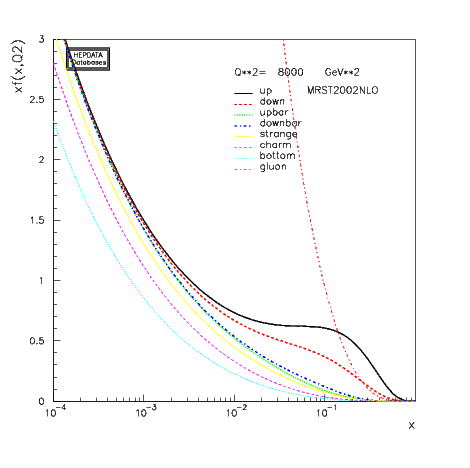
\includegraphics[scale=0.5]{THESISPLOTS/PDF_TEN.png}
%\captionof{figure}{Pdfs.}
%\label{fig:pdfs}
%\end{center}

%It is imperative to know the uncertainty in the measurement of PDFs as this is usually a source of uncertainty in a related experiment.
%%%%%%%%%%%%%%%%%%%%%%%%%%%%%%%%%%%%%%%%%%%%%%%%%%%%%%%%%%%%%%


%\newline
%The value of the strong coupling $\alpha_{S}$ which determines the strength of the strong interaction depends on the momentum transfer $Q^{2}$ as do the coupling constants of the $SU(2) \times U(1)_{Y}$ groups.
% For large $Q^{2}$, $\alpha_{S}$ approaches zero in a process in QCD referred  to as \textit{asymptotic freedom} and the quarks are nearly free while for small values of $Q^{2}$, $\alpha_{S}$ grows large and the quarks are tightly bound. This process is also referred to as \textit{confinement}.
%Quarks are always confined to hadronic bound states called baryons or mesons consisting of three quarks or a quark and anti-quark respectively.
%\newline
%The proton is the most stable baryon. It is made up of two up quarks and one down quark such that its electric charge is 1. These are called valence quarks. It turns out that from experiments, valence quarks are not the only quarks present in a proton. Infact it is best to describe the proton as made up of \textit{partons}. Partons are quarks and gluons. 
%Inside a proton, it is possible for a gluon to radiate or split up into a quark anti-quark pair. These kind of quarks are referred to as sea quarks. All partons in a proton carry the total momentum of the proton, however during proton-proton collision in a hadron accelerator, the partons are the actual colliding particles and not the protons so it is imperative to know the momentum fraction \textit{x} of an individual parton inside a proton. The momentum fraction of a parton is expressed as a \textit{Parton Distribution Functions}~(PDFs).

% very well when performing a search for physics beyond the SM as calculating scattering \textit{cross sections} which is an experimentally observable quantity describing the probability of a particular process happening highly depends on PDFs. In addition to this, due to the PDFs, the center of mass for proton-proton collision which in actual experiment is parton-parton collision is much reduced from $\sqrt{S} = 14$ \TeV as advertised in the LHC to $\sqrt{\hat{s}} \approx 2$ \TeV and this depends on the particular partons involved in the parton-parton interaction.


%\paragraph*{}
%Without the Higgs mechanism, all the particles described so far will be massless. But experiments observe massive particles, So how do we get these particles to have mass in the SM?
%This questions remains and important one in particle physics. However in the case of the SM, we obtain mass by "manually" breaking the gauge symmetries in the SM through the addition of mass terms into the SM Lagrangian. Thus the introduction of mass terms through the Higgs mechanism breaks the local gauge invariance in the theory which describes all the above interactions.
\subsection{Spontaneous Symmetry Breaking}
\textit{Spontaneous symmetry breaking} is the spontaneous breaking of the gauge symmetry from a parent symmetry into an entirely, new sub-symmetry. In the SM, spontaneous symmetry is realized as represented by the expression in equation \ref{eq:SYMB}.
\begin{equation}{\label{eq:SYMB}}
 SU(3)_{C} \otimes SU(2)_{L} \otimes U(1)_{Y} \xRightarrow{SSB~into} SU(3)_C \otimes U(1)_{QED}
\end{equation}
Early attempts prior to the 1960s to construct a gauge theory of weak interactions failed because the gauge bosons were massless while experimental evidence proved otherwise.
% Which indicated that the strength of the weak interaction can be infinite just like the electromagnetic interactions. However, theories were in complete contrast with results from experiments as weak interactions were understood to be limited to very small distances of about the scale of the nucleus. Thus these massless gauge bosons had to become massive.
%\paragraph*{}
\newline
The Higgs~(or Higgs-Brout-Englert) mechanism \cite{HIGGS}, is achieved by introducing a complex weak isospin \textit{scalar doublet}, $\mathbf{\phi}$, i.e spin $s = 0\hbar$.
During this process, the  $SU(2)_{L} \otimes U(1)_{Y}$ symmetry is spontaneously broken into a $U(1)$ symmetry  which describes electromagnetic interaction. Figure \ref{fig:Higgs} shows a picture of the potential of the spin-$0$ complex Higgs field.
The minimum value of the potential, $|\phi_{0}| = \sqrt{\frac{-\mu^{2}}{\lambda}}  = \nu $, based on the choice of the parameters $\mu^{2} < 0 $ and $ \lambda > 0$, is to spontaneously break the $SU(2)_{L} \otimes U(1)_{Y}$ symmetry into $U(1)$ symmetry.  During spontaneous symmetry breaking, both matter and gauge bosons, except the photon~{\Pphoton), obtain masses. The process is referred to as \textit{Higgs-Brout-Englert mechanism} or \textit{Higgs mechanism}.
%\begin{equation}
%INSERT HIGGS DOUBLET HERE 
%\end{equation}

%which is invariant under the gauge symmetry group $SU(2)_{L} \times U(1)_{Y} $  and has its dynamics described by the Lagrangian density:
%\begin{equation}
% HIGGS DOUBLET LAGRANGIAN
%\end{equation}

% responsib is the Higgs doublet with spin-0 complex components.
%The parameter $\mu^{2} < 0 $ and the real parameter $\lambda > 0$ of the scalar Higgs potential(figure \ref{fig:Higgs}).

%is chosen such that the potential $V \rightarrow \infty $ as $\mathbf{\Phi} \rightarrow  0 $.
%It is easily seen from the previous equation that the minimum of the potential is not longer at $\mathbf{\Phi} = 0 $ but  lies at :



%With this choice of parameters settings, the potential V is itself $SU(2)_{L}$ symmetric but any other choice of ground state breaks $SU(2)_{L}$ symmetry. This is referred to as the \textit{Higgs-Brout-Englert mechanism} or \textit{Higgs mechanism} for simplicity.
%This choice of parameters of the potential V can be seen in figure below.

%\begin{equation}
%put higgs potential picture in here!
%\end{equation}

%One can then choose $\phi_{1} = \phi_{2}= \phi_{3} = 0$ and then parametrise the higgs doublet as small perturbations around the minimum as follows:
%\begin{equation}
%equation of higgs pertubations
%\end{equation}
%with $h(x), \eta_{i}(x)$ being 4 real scaler fields. Using the gauge freedom of $SU(2)_{L} \times U(1)_{Y}$ once can choose the \textit{unitarity gauge} where the kinetic terms for the fields $\eta_{i}(x)$ vanish and their with the requirement of local gauge invariance, $\eta_{i}(x)$ couple to the massless gauge bosons to be to become massive and the resulting Higgs doublet is expressed as:
%\begin{equation}
%Higgs doublet with imaginary parts removed
%\end{equation}
%With the imaginary parts removed and the  field $h(x)$ is identified as the physical real scalar Higgs field or Higgs boson.
%The ground state chosen so that the photon remains massless while the other gauge bosons including the real scalar Higgs field are massive with their masses given as:
%\begin{equation}
%Eqns of Gauge boson masses and Higgs mass
%\end{equation}
%The $Z^{0}$ mass $m_{Z}$ can also be expressed in terms of the $W^{\pm}$ mass $m_{W}$ and the Weinberg angle as:
%\begin{equation}
% Z mass to W mass equation
%\end{equation}
%Thus one can easily observe that all the effects of the W and Z bosons can be described in terms of the parameters $e$, $\theta_{w}$ and $\nu$ which can be expressed in term of Fermi constant all of which were experimentally known. Thus it is fine to say that the Higgs mechanism could predict the masses of W and Z gauge bosons which were experimentally found and measured in 1983 at LEP\cite{}.This discovery was one of the greatest triumphs of the SM.
%With the value of $\nu \approx 246$~GeV, we can then express the mass of the fermions in terms of the Yukawa coupling as ( from the Yukawa sector of the Lagrangian) :
Quarks and leptons obtain their masses through their interaction with the Higgs field.
A fermion's mass, $m_{f}$, is proportional to the strength of its interaction (\text{Yukawa} coupling $\lambda_{f}$) with the Higgs field. Electro-weak interaction mediating gauge bosons, $\PZzero$ and $\PWpm$ obtain their mass $m_{Z}$ and  $m_{\PWpm}$, respectively, by engulfing or "\textit{eating}" the available massless components~(\textit{Nambu-Goldstone bosons}) of the complex Higgs doublet.
From the four scalar fields(complex Higgs doublet), only a physically massive \textit{Higgs boson} remains.
\begin{equation}
m_{f} = \lambda_{f}\frac{\nu}{\sqrt{2}}, \quad \quad  \frac{m_{W^{\pm}}}{ m_{Z}} = \frac{\frac{1}{2}\nu g}{\frac{1}{2}\nu\sqrt{g^{2} + {g^{\prime}}^{2}}} = \cos\theta_{w}
\end{equation} 
The search for the Higgs boson was one of the purpose for building the large hadron collider at CERN.
The discovery of the Higgs candidate scalar boson through its decay into two photons, \HGG, and a pair of $\PZ$ bosons, $\PHiggs\rightarrow \PZ\PZ $,  was presented to the public on July 04, 2012. Its  measured mass was $m_{H} = 125\pm 0.21$\GeVcc.
\newline
It is important to note that there is no fundamental reason given by the SM why there should be only one type of the Higgs field to which all fermions couple to obtain their masses nor any prediction from the SM for the choice of parameters.
There are other models such as supersymmetry, which allows for the possibility of more than one Higgs field.
In Figure \ref{fig:ALLSM}, we show a complete summary of particles and their interactions as described by the SM.


\begin{center}
\centering
%\mbox{
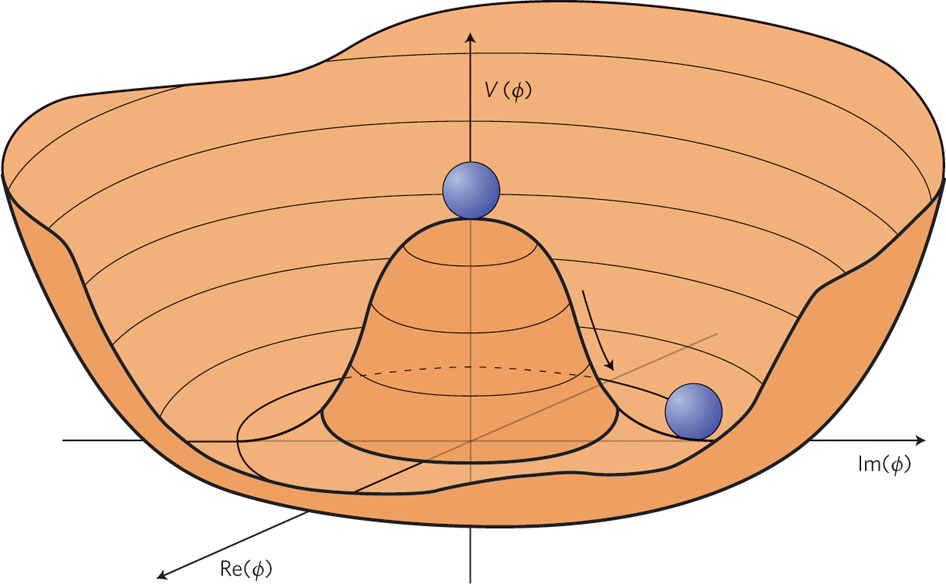
\includegraphics[scale=0.25]{THESISPLOTS/Higgs_Potential.jpg}
\captionof{figure}{Higgs boson "Mexican hat" potential, $V(\phi^{*}\phi) = \mu^{2}(\phi^{*}\phi) + \lambda(\phi^{*}\phi)^{2}$, which leads to spontaneous symmetry breaking with choice of parameters $\mu^{2} < 0$, $\lambda > 0$.}
\label{fig:Higgs}
\end{center}

\begin{center}
\centering
%\mbox{
%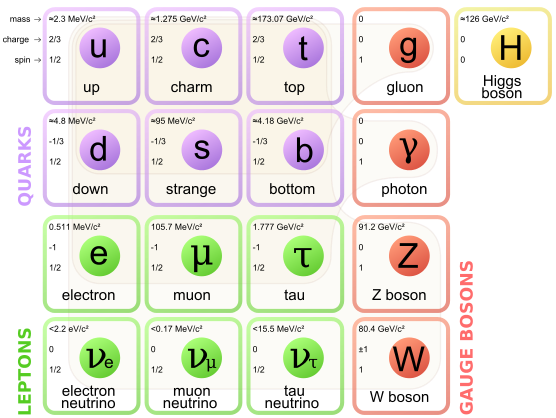
\includegraphics[scale=0.5]{THESISPLOTS/Standard_Model_of_Elementary_Particles.png} 
%\vspace{1cm} 
%\quad
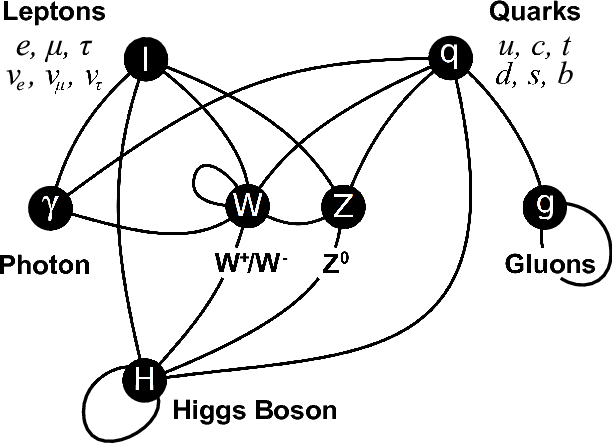
\includegraphics[scale=0.5]{THESISPLOTS/SM_Particles.png}%}
\captionof{figure}{SM particles and their interactions with vector bosons as mediators.}
\label{fig:ALLSM}
\end{center}

\clearpage

\subsection{Limitations of the Standard Model }
Although numerous experiments support the SM in its description of particle properties with unmatched precision, there are many unanswered questions by the SM. We provide a summary below of those of our interest.
%~(Glashow, 1961; Weinberg, 1967; Salam, 1968) describes almost entirely all of the observed phenomena and fundamental particles of nature with unmatched precision.
%However, more concerning our universe is yet to be understood. A few of this include:
\begin{itemize}
\item \textbf{General Formalism} \mbox{}\\ Many important parameters like particle masses, Weinberg angle, the CKM matrix elements, for example, cannot not be derived from the SM. These are measured from experiments. Why only 3 generations of particles? 
Why the specific doublet representation of fields in the SM? These are questions to which the SM provides no answer.
%The Electro-weak symmetry breaking which is central to the SM is not very well understood as the SM does not provide an explanation of whether there are more than one spin-0 boson responsible for particles masses or not.

\item \textbf{Cosmological} \mbox{}\\
Why is there so much matter than anti-matter in the universe? \textit{Cosmic Microwave Background}~(CMB) and the \textit{Wilkinson Microwave Anisotropy Probe}~(WMAP) experimental results indicate the presence of excess matter which does not interact with light called \textit{Dark Matter}~(DM) and \textit{Dark Energy}~(DE). DE is responsible for the increase energy density causing rapid accelerating expansion  of the universe. The nature of DM and DE and such observations cannot be explained using the current SM.
%If the Big Bang theory which describes the creation and existence of the universe is assumed to be the correct theory, then matter and anti-matter should be observed in equal composition. However, astrophysical measurements of the ratio of barons to anti-baryons referred as the \textit{Baryon asymmetry ratio} shows that there is more matter than anti-matter in the universe. Where is all the expected anti-matter? This could fairly be explained through charge-parity violation in weak interactions of the SM but this contribution is not enough to explain the entire observed baryonic matter discrepancy. Observations through \textit{Baryonic Acoustic Oscillation}~(BAO) or .
\item \textbf{Theory} \mbox{}\\
SM description of nature does not include gravitational interactions.
Observation of SM coupling constants varying with energy begs the question of whether at some higher energy scale, all the weak, strong and electromagnetic coupling constants behave as one i.e unified as a single coupling constant. If possible, at what energy scale does this force unification occur?

\item \textbf{Mass Hierarchy or Naturalness} \mbox{}\\
Particle masses ranges from neutrino masses, a few eV to the \textsf{top} particle's mass of 173~\GeVcc.
The SM does not explain this mass hierarchy.
To some physicist, the energy gap between the electro-weak symmetry breaking energy scale~( $\approx 246$~\GeV) and the Planck energy scale~(reduced Planck mass, $M_{p} = 10^{18}$~\GeV) seems unnatural.

% The SM only accounts for how particles obtain their mass through their interaction with a scalar field~(spin-0), the Higgs boson. However, the experimental observation of this particles mass hierarchy is not understood. Infact according to the SM, neutrinos have no mass. 
%From an energy scale point of view, this lack of our understand also known as the \textit{hierarchy} "\textit{problem}" can be posed as follows; why do experiments observed such a 
%A consequence of this, is on the experimentally observed value of the mass of the Higgs boson, $\approx 125$~\GeV. The Higg's mass is stable and does not grow to very large values as the energy scale increases towards $M_{p}$ as one would expect from theoretical calculations.  \textit{Supersymmetry}, an extension of the SM, allowing for the possibility of more than a single Higgs boson, provides an explanation for why the  Higg's mass remains stable at all energy scale. Its main idea, is the existence of fundamental new particles with masses within the weak and gravity energy scale and through their interaction with the higgs keeps its mass stable. We will see more of this in the next section.
\end{itemize}
%%%%%%%%%%%%%%%%%%%%%%%%%%%%%%%%%%%%%%%

\section{Beyond Standard Model Physics}
%%%%%%%%%%%%%%%%%%%%%%%%%%%%%%%%%%%%%%%
%The SM predictions of the value of the Higgs boson's mass recommend additional contributions from \textit{quantum fluctuations}~(higher order or loop corrections) which are very large~(can as well be infinite). However, the observed experimentally measured value of the Higgs mass~($m_{H} \approx 125$~\GeV). This unobserved large corrections to the experimentally measured value requires some understanding. A possible explanation is that these various contributions cancel on average producing a net zero effect on the true Higgs mass such that the physically observed mass is as measured. If such cancellation is a true phenomenon in nature, then it is only logical to inquire the origin of this cancellations. Obviously this cannot be understood within the frame work of the SM. 

%Consequently, theories beyond the SM like \textit{supersymmetry} provide a natural understanding of how these various contributions cancel on average arriving at the physically observed and measured Higgs mass. To expand further, the mass of a particle can be expressed as 
%\begin{equation}
% m^{2}_{\mbox{physical}} = m^{2}_{\mbox{bare}} + \delta m^{2}_{1}
%\end{equation}

%where $m^{2}_{\mbox{physical}}$ is the physically measured mass of the Higgs boson,  $m^{2}_{\mbox{bare}}$ is the true  universe given mass of the particle which cannot be calculated or measured. $\delta m^{2}_{1}$ are corrections from quantum fluctuations to the true mass which can be calculated. Using the measured mass and the calculated  quantum corrections, one can obtain the true Higgs mass. These contributions from quantum fluctuations can arise from both bosons and fermions. Since the Higgs boson can interact~(by coupling) with every particle through interactions of the general form $\lambda_{f}H\bar{f}f$ for fermions and $\lambda_{S}|H|^{2}S^{2}$ for scalar or bosons;  with $\lambda_{f}$ and $\lambda_{S}$ representing the coupling constants which need not be equal. The Feynman diagrams in \ref{fig:Hmass} represents a few of such quantum fluctuations with both fermion and boson contributions computed as:
%Putting Figures side by side.
The Higgs boson mass from SM predictions include additional corrections,$\delta m^{2}$, to the higgs mass through its couplings with fermions such as the diagram shown in Figure \ref{fig:HM}(a). These additional corrections are given as shown in equation \ref{eq:HFermion}.

\begin{equation}{\label{eq:HFermion}}
\delta m^{2}_{f} = \frac{1}{16\pi^{2}}|\lambda_{f}|^{2}\left(-2\Lambda^{2} + 6m^{2}_{f}\ln\left(\frac{\Lambda}{m_{f}}\right) + ...\right) 
\end{equation}
Where $\lambda_{f}$ is the Higgs to fermion coupling, $\lambda_{f}H\bar{f}f$ and $\Lambda$ is an arbitrarily large energy scale~(can be of order $10^{18}$\GeV) called the \textit{cut-off} energy scale. 
 As a result of this cut-off scale being very large, these corrections can also be very large.
However, large corrections to the Higgs boson's mass are not observed in experimental measurements of the Higgs boson's mass which is $125$~\GeVcc.
The SM provides no explanation for why these corrections are not observed.
\begin{center}
%\begin{figure}[ht]
\begin{minipage}[b]{0.45\linewidth}
\centering
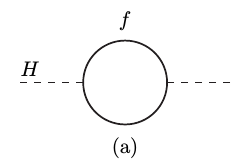
\includegraphics[width=0.70\textwidth]{THESISPLOTS/Higgs_MassFermion.png}
%\captionof{figure}{Higgs fermion coupling}
%\label{fig:HMassL}
\end{minipage}
\hspace{0.5cm}
\begin{minipage}[b]{0.45\linewidth}
\centering
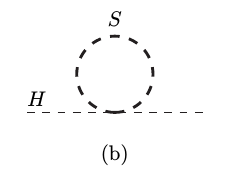
\includegraphics[width=0.70\textwidth]{THESISPLOTS/Higgs_MassScalar.png}
%\caption{Higgs scalar coupling}
%\label{fig:HMassL}
\end{minipage}
%\end{figure}
\captionof{figure}{Higgs mass contributions from its coupling to fermions~(a) and scalar~(b) fields.}
\label{fig:HM}
\end{center}
%\begin{center}
%\centering
%\mbox{
%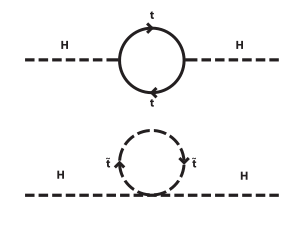
\includegraphics[height=5cm,width=0.5\linewidth]{THESISPLOTS/Higgs_Hirrachy_Problem.png}
%\captionof{figure}{Higgs self energy diagrams showing how the higgs boson mass is computed from both Higgs field and supersymmetric partner particle contributions.}
%\label{fig:Hmass}
%\end{center}
Models beyond the SM like \textit{supersymmetry}, provide a plausible explanation as to why these corrections are not observed in experiments.  The explanations is that, there are in addition to the higgs boson being the only scalar particle in the SM,
new  scalar particles, yet to be observed, which can also couple to the higgs field as shown in the diagram in figure \ref{fig:HM}(b). These scalar coupling contribution, given in equation \ref{eq:HScalar} is of the opposite sign and as a result cancel the fermion contributions to the Higgs boson's mass. This is the explanation why the corrections to the Higg Boson's mass cannot be observed experimentally.
\begin{equation}{\label{eq:HScalar}}
\delta m^{2}_{S} = \frac{1}{16\pi^{2}}|\lambda_{S}|^{2}\left(\Lambda^{2} - 2m^{2}_{S}\ln\left(\frac{\Lambda}{m_{S}}\right) + ...\right) 
\end{equation}
This problem is known as the \textit{Hierarchy problem} and is explained using suppersymmetry. This cancellation is provided
at all levels of the Higgs boson interaction and for whatever energy scale the cut-off value may be.
%$\Lambda$ is some \textit{cut-off} energy scale where a another kind of physics interaction like gravity at a much higher energy scale is needed to regulate the low energy behavior of the SM. $\Lambda$ could be the reduced Planck scale(~ $10^{18}$~\GeV).  A quick observation from this calculations is that; first, corrections to the higgs bare mass, $m^{2}_{\mbox{bare}}$ are not proportional to the Higgs mass.
%( in other cases like as is the case with other SM particles like the electron\cite{}.
%Second, these corrections are of the order of $\approx 10^{36}~\GeV^{2}$  bringing positive and negative contributions from fermions or scalar bosons respectively.
%Even with these corrections to the true Higgs mass, the measured~(physical) Higgs mass squared, $m^{2}_{H,\mbox{physical}}$, is of the order $\approx 10^{4}~\GeV^{2}$.
%Since the true Higgs mass, $m^{2}_{H,\mbox{bare}}$, is never measured or known, an agreement between these quantum fluctuation contributions and physical Higgs mass is realized  if only the true Higgs mass, $m^{2}_{H,\mbox{bare}}$,  is \textit{fine-tuned} with a precision of about 1 in $10^{17}$. This enormous fine-tuning is considered a fundamental issue of not enough understanding of the Higgs mechanism of the SM and is considered \textit{unnatural}. 
%The fact that, among the numerous SM predictions, no other scalar particle except the possible Higgs boson candidate has been observed so far, further makes such a fine-tuning difficult to understood. 
%On the other hand, in suppersymmetry, the fermion one loop quantum correction which comes with an opposite sign to the scalar quantum fluctuation corrections and $\lambda_{f} = \lambda_{S}$ ,there is a complete  cancellation and this discrepancy of the unobserved effects of these quantum fluctuations to the $m^{2}_{H,\mbox{bare}}$ in the $m^{2}_{H,\mbox{physical}}$ is understood. 
% Another interpretation of this issue is through the question of why there is so much difference in energy scale between the electroweak scale \textit{O}(100~\GeV) and the Planck energy scale \textit{O}($10^{19}$~\GeV) where gravity effects to particle interaction becomes significant?. This is referred to as the \textit{Hierarchy problem} stated above as one of the motivation to go beyond SM.
Supersymmetry does not only provide an explanation to the Hierarchy problem, but also provide a good framework for
the unification of fundamental forces. In addition, supersymmetry also predicts the existence of additional particles to the SM which are
non interacting with ordinary matter and having very long lifetime making these particles exceptional candidates as dark matter
particles. These properties motivates the study of supersymmetry as an interesting extension of the SM for understanding
physics beyond the SM~(BSM).
%In addition to explaining the origin of this perceived \textit{fine-tuning} issue, supersymmetry also provides a natural framework for the unification of fundamental forces, not possible in the SM.
%If the SM is believed to be an incomplete and low energy description of nature of a possible parent and more fundamental theory like supersymmetry, then one would expect that the symmetry groups of the SM be a subset of some larger parent group, $\mathcal{G}$; i.e $\displaystyle{SU(3)_{C} \otimes SU(2)_{L} \otimes U(1)_{Y} \subset \mathcal{G}}$.
%It is believed that at a higher energy scale since SM seems to be describing the  behavior of some parent theory, the electromagnetic, weak and strong interactions all become one interaction just as the electromagnetic and weak interaction unified into the electro-weak interaction as the electro-weak energy scale $\approx 100$~\GeV. i.e
%$\mathcal{G}$ is some larger symmetry group. In SM, this does not happen at any higher energy scale. However, in 
%In suppersymmetry, This unification of forces or couplings of electromagnetic, weak and strong interactions occur at the \textit{Grand Unified Energy}~(GUT) energy scale of $\approx 10^{15}$~\GeV \cite{SM}.
%This effect can be seen in the following figures as taken from \cite{}.
%\begin{equation}
%Plot showing Unification of Coupling Constants.
%\end{equation}
%%\clearpage
%%%%%%%%%%%%%%%%%%%%%%%%%%%%%%%%%%%%%%%%%%%%%%%%%%%%%%%%%%%%%%%%%%%%%%%%%%%%%%%%%%
%%%%%%%%%%%%%%%%%%%%%%%%%%%%%%%%%%%%%%%%%%%%%%%%%%%%%%%%%%%%%%%%%%%%%%%%%%%%%%%%%%
\subsection{Supersymmetry}
%%%%%%%%%%%%%%%%%%%%%%%%%%%%%%%%%%%%%
Suppersymmetry is a relativistic Quantum Field Theory~(QFT), relating space-time symmetries~(rotation and translation) and 
gauge symmetries~($SU(3)_{C}\otimes SU(2)_{L}\otimes U(1)_{Y}$).
During the early period, very little was understood about supersymmetry. Progress in understanding began with the \textit{Haag-Lapuszanski-Sohnius} theorem \cite{MSUSY} in 1975. This led to the introduction of supersymmetry generators called \textit{Lie-superalgebra} generators, $\mathrm{Q}_{i}$, $i = 1,...,\mathrm{N}$, where $\mathrm{N}$ is the number of supersymmetry generators, which anti-commute  with the group and space-time generators. The consequence is that fermions can be transformed into bosons and vice-versa. This boson-to-fermion and fermion-to-boson transformation is expressing using Equations \ref{eq:SUSY}.
\begin{eqnarray}{\label{eq:SUSY}}
\mathrm{Q}|\textbf{Fermion}\rangle =|\textbf{Boson}\rangle,    &
\mathrm{Q}|\textbf{Boson}\rangle  =|\textbf{Fermion} \rangle 
\end{eqnarray}
Thus, in supersymmetry, particles in a given state  have the \textit{same} mass but differ in their spin by half $\hbar$ and in every irreducible representation of supersymmetry, like the chiral representation, there is an equal number of fermionic and bosonic degrees of freedom. Every particle has a supersymmetric partner with the same mass belonging to the same  state representation or \textit{supermultiplet}.

%In relativistic Quantum Field Theory~(QFT), the idea of symmetry or group theory is used to provide a better understanding of fundamental particles and their properties. These symmetries belong to two broad categories: space-time symmetries known as Poincar\'{e}(i.e rotation and translation) symmetries and gauge ( such as $SU(3)_{C}\otimes SU(2)_{L}\otimes U(1)_{Y}$ with quantum numbers; color, weak and hypercharge respectively of the SM) symmetries. With the SM viewed as a low energy version of a more large and unified theory,  
%that all fundamental forces including gravity could be unified 
%In a quest to include gravitational interaction along with all the other forces of nature into a unique frame work called unification, 
%it was believed that combining these two classes of symmetries into one big class of symmetry could lead the way towards the development of this unified theory. However, Coleman and Mandula\cite{SUSY}, in their so-called "\textit{no-go}" theorem in 1967  showed that pursuing the approach of \textit{direct product} of the two super groups  was not possible. %Thus these two class of symmetries cannot be combined into a bigger parent symmetry. 
%The challenge was finding a scenario where the generators of both space-time $P^{\mu}$, $M^{\mu\nu} $  and gauge groups $T^{a}$, do not commute with each other; i.e $ \left[M^{\mu\nu}, T^{a}\right] \neq 0$ and yet remains a direct product of both symmetry groups, considering that the direct product of these groups do commute; i.e
%the generators of these groups; $P^{\mu}, M^{\mu\nu}$ and $T^{a}$ corresponding to these symmetries have a direct product;  Poincar\'{e} $\times$Gauge group, for which
%$ \left[P^{\mu}, T^{a}\right] = \left[M^{\mu\nu}, T^{a}\right] = 0$. 
%\newline
%This \textit{no-go} theorem prevents the possibility of finding a parent group where its generators are constructed from \textit{Lorentz} tensors. Thus, only symmetries  generated from \textit{spinoral}~(particle's spin) charges instead of \textit{tensorial}~(space-time) charges were possible. In 1975, Haag, Lapuszanski and Sohnius \cite{MSUSY} found such a group theorem known as the \textit{Haag-Lapuszanski-Sohnius} theorem with its corresponding generator algebra called the \textit{Lie-superalgebra} or the \textit{supersymmetry algebra}.  This supersymmetry algebra extended the commutative aspect of the Poincar\'{e} algebra to include \textit{anticommuting} symmetry generators.
%\newline
%\textit{Lie-superalgebra} generators, $\mathrm{Q}_{i}$, $i = 1,...,\mathrm{N}$, where $\mathrm{N}$ is the number of supersymmetry generators, anti-cummute with the group and space-time generators.  % as shown in equation \ref{eq:SUSYGEN}. 
%Supersymmetry is a well developed and advanced branch in theoretical physics where the number of supersymmetry generators can be any number. However, this thesis only considers the case where there is only one generator of supersymmetry; i.e $\mathrm{N} = 1$. This is the minimal  version of supersymmetry. 
% The generators $\mathrm{Q_{1}} \equiv \mathrm{Q^{\alpha}}$, where $\alpha=1,2$ is labeling \textit{Weyl or two spinor} components,  and its hermitian conjugate, $\mathrm{\bar{Q}_{\alpha}}$, must satisfy the relations given in equation \ref{eq:SUSYGEN}.
%\begin{eqnarray}{\label{eq:SUSYGEN}}             
%\left\lbrace\mathrm{Q_{\alpha}}, \mathrm{\bar{Q}_{\beta}}\right\rbrace =  2\left(\gamma^{\mu}\right)_{\alpha\beta}P^{\mu}, &
%\left[\mathrm{Q_{\alpha}},P^{\mu}\right] = 0, &
%\left[\mathrm{Q_{\alpha}}, M^{\mu\nu}\right] =\frac{1}{2}\left(\Sigma^{\mu\nu}\right)_{\alpha}^{\beta}\mathrm{Q_{\beta}}
%\end{eqnarray}
%$\gamma^{\mu}$ is define such that 
%Where $\left\lbrace \gamma^{\mu}, \gamma^{\nu}\right\rbrace = 2\mathrm{g^{\mu\nu}}$ and  $\Sigma^{\mu\nu} = \frac{i}{2}\left[\gamma^{\mu},\gamma^{\nu}\right]$ 
%. %and $\mathrm{\bar{Q}_{\alpha}}$ is the Hermitian conjugate to $\mathrm{Q}$.
%These relations in equation \ref{eq:SUSYGEN} reveal two very fundamental consequences of supersymmetry:
%\begin{itemize}
%\item  Particles in a given state~(\textit{supermultiplet}) have the same mass but differ in their spin by half $\hbar$ unit.
%\item In every irreducible representation of supersymmetry, there is an equal number of fermionic and bosonic degrees of freedom. 
%\end{itemize}
%Thus, supersymmetry is the symmetry which transforms particles from one spin into another with the same mass. As a consequence, supersymmetry generators transform fermions into bosons and bosons into fermions with the same mass.

%This reveals that, in supersymmetry, 
% chosen such that every SM particle with spin 0,$\frac{1}{2}$, 1, 2 have a partner with spin $\frac{1}{2}$,0,$\frac{1}{2}$,$\frac{3}{2}$ respectively in the same supermultiplets.
These supermultiplets are either \textit{Chiral}, \textit{Vector} or \textit{Gravity} multiplets. The minimal supersymmetric extension of SM uses Chiral and Vector supermultiplets shown in Table \ref{tab:SUSYM}.

\begin{center}
\centering
%\bfseries{Supersymmetry multipletes and spin }
\begin{tabular}{c |c|c}
\toprule
\bfseries{Supermultiplets} & \bfseries {Spin in SM}, & \bfseries{Spin in Supersymmetry}\\
\hline
\textit{Chiral} & $0$ & $\frac{1}{2}$ \\ 
\textit{Chiral} &$\frac{1}{2}$ & $0$ \\   \hline
\textit{Vector} & $1$ & $\frac{1}{2} $ \\ \hline
\textit{Gravity} & $2$ & $\frac{3}{2} $ \\
\hline 
\bottomrule
\end{tabular}
\captionof{table}{Supermultiplets and particle spin in SM and Supersymmetry.}
\label{tab:SUSYM} 
\end{center}

Models in supersymmetry are developed using \textit{superfields}, \textbf{$\Phi$}. A given superfield consists of
ordinary scalar real or complex fields~($\phi$), a Lorentz vector field~($ A_{\mu} $) and Left-handed or Right-Handed Weyl(2 degrees of freedom) spinor fields~($\psi$). \textit{Chiral} and \textit{Vector} superfields are used in constructing the minimal supersymmetric standard model.
%In addition to an algebraic approach to supersymmetry described so far, in order to build models~(supersymmetric Lagrangians) and make predictions, we return to the idea of fields as used in supersymmetry. Supersymmetric fields are called \textit{superfields}~( proposed and realized by Abdus Salam and Strathdee \cite{SALAM, SUSYBOOK}) are fields defined on a superspace; an ordinary Minkowski space-time, $x^{\mu}$ and four anti-commuting \textit{Grassmann} numbers, $\theta$. More on this can be seen in  \cite{SUSYBOOK}.
%These superfields are operator-valued functions, \textbf{$\Phi$}, on a superspace represented by, \textbf{$\Phi\left(x^{\mu},\theta,\bar{\theta}\right)$}.
%Its components consist of ordinary scalar fields~(real or complex), Lorentz vector fields and Left-handed or Right-Handed Weyl(2 degrees of freedom) spinor fields, \textbf{$\Phi\left(x^{\mu},\theta,\bar{\theta}\right) \supset (\phi, \psi, A_{\mu}, F)$}.
%Table \ref{tab:SUSYF} shows an example of the components which make up the  superfield~( or supermultiplets) with each component representing a SM particle and its super partner with the same mass. Only the Chiral and Vector  superfields are used in constructing the minimal supersymmetric version of standard model
%\begin{center}
%\centering
%\begin{tabular}{|c| c|}
%\mbox{Supersymmetry multipletes and spin }
%\hline
%\bfseries{Superfields or supermultipltes } & \bfseries {Component Fields}\\
%\hline
%\textit{Chiral} & $(\psi, \phi, F)$ \\
%\textit{Vector} & $(A_{\mu},\lambda, D)$ \\
%\textit{Gravity} & $ (G_{\mu\nu}, ... ) $ \\
%\hline \hline
%\end{tabular}
%\captionof{table}{Supermultiplets and components in Supersymmetry.}
%\label{tab:SUSYF} 
%\end{center}
The simplest supersymmetric model is an extension of the SM to include supersymmetric particles with the same mass
as their standard model partners. It is called the \textit{Minimal Supersymmetric Standard Model} because it only involves the 
use of a single supersymmetry generator.

\subsection{Minimal Supersymmetric Standard Model}
In the Minimal Supersymmetric Standard Model~(MSSM), the number of fundamental particles is increased.
The full particle content in MSSM with this extension from SM is shown in Table \ref{tab:SUSYP} and \ref{tab:SUSYG}.
\newline
The nomenclature of supersymmetric particles is derived from their SM counterparts by adding an "\textit{s}" in front of the 
SM particles names. For example, a \textit{selectron} is the supersymmetric partner of the electron, \textit{squarks} are the supersymmetric partners of SM quarks. There are exceptions to this nomenclature which we will mentioned later. 
Both supersymmetry particles and their SM partners should have the equal masses, however,
there have been no experimental evidence for such supersymmetric particles having the same mass as SM particles. Therefore,
Supersymmetry is definitely not an exact symmetry in nature and must be spontaneously broken. 
\begin{center}
\centering
\begin{tabular}{l |l| l| l| l}
%\mbox{Supersymmetry multipletes and spin }
\toprule
\bfseries{Particle Names} &\bfseries{Symbol}  & \bfseries {spin 0} & \bfseries{spin 1/2} & \bfseries{$SU(3)_{C}\otimes SU(2)_{L}\otimes U(1)_{Y}$} \\
\hline \hline
\vtop{\hbox{\strut{ squarks, quarks}}
\hbox{\strut{($ \times 3$ families)}}} & $Q$ & $(\tilde{u_{L}}, \tilde{d_{L}})$ & $(u_{L}, d_{L})$ & $(\mathbf{3}, \mathbf{2}, \frac{1}{6})$ \\
    & $\bar{u}$ & $\tilde{u}^{\star}_{R}$ & $u^{\dagger}_{R}$ &
   $(\bar{\mathbf{3}}, \mathbf{1}, -\frac{2}{3})$ \\
     &  $\bar{d}$ & $\tilde{d}^{\star}_{R}$ & $d^{\dagger}_{R}$ &
   $(\bar{\mathbf{3}}, \mathbf{1}, \frac{1}{3})$ \\
   \hline
 \vtop{\hbox{\strut{ sleptons, leptons}}
\hbox{\strut{($ \times 3$ families)}}} & $L$ & $(\tilde{\nu}, \tilde{e_{L}})$ & $(\nu, e_{L})$ & $(\mathbf{1}, \mathbf{2}, -\frac{1}{2})$ \\

& $\bar{e}$ & $\tilde{e}^{\star}_{R}$ & $e^{\dagger}_{R}$ &
   $(\bar{\mathbf{1}}, \mathbf{1}, 1)$  \\
   \hline 
higgsinos, Higgs & $H_{u}$ & $(H^{+}_{u}, H^{\circ}_{u})$ & $(\tilde{H}^{+}_{u}, \tilde{H}^{\circ}_{u})$ & $(\mathbf{1}, \mathbf{2}, +\frac{1}{2})$ \\   
   & $H_{d}$ & $(H^{\circ}_{d}, H^{-}_{d})$ & $(\tilde{H}^{\circ}_{d}, \tilde{H}^{-}_{d})$ & $(\mathbf{1}, \mathbf{2}, -\frac{1}{2})$  \\ 
\hline
\bottomrule
\end{tabular}
\captionof{table}{Chiral supermultiplets and representation in Minimal Supersymmetric SM~(MSSM). Super symmetric particles~(sparticles) have a $\tilde{•}$ on them. Spin -0 fields are complex scalars while spin-1/2 fields are left-handed two component Weyl fermions.}
\label{tab:SUSYP} 
\end{center}

\begin{center}
\centering
\begin{tabular}{l|l| l| l}
%\mbox{Supersymmetry multipletes and spin }
\toprule
\bfseries{Particle Names} & \bfseries {spin 1/2} & \bfseries{spin 1} & \bfseries{$SU(3)_{C}\otimes SU(2)_{L}\otimes U(1)_{Y}$} \\
\hline \hline
gluino, gluon & $\tilde{g}$  & $g$ &  $(\mathbf{8}, \mathbf{1}, 0)$ \\
\hline
winos, $W$ bosons & $\tilde{W}^{\pm}, \tilde{W}^{\circ}$ & $W^{\pm}, W^{\circ}$ & $(\mathbf{1}, \mathbf{3}, 0)$ \\
\hline
bino, $B$ boson & $\tilde{B}^{\circ}$ & $ B^{\circ}$  & $(\mathbf{1}, \mathbf{1}, 0)$ \\
\hline 
\bottomrule
\end{tabular}
\captionof{table}{Gauge supermultiplets and representations in Minimal Supersymmetric SM~(MSSM). Super symmetric particles~(sparticles) have a $\tilde{•}$ on them.}
\label{tab:SUSYG} 
\end{center}

%In order for supersymmetry~(SUSY) predictions to be agreement with observations from experiments, SUSY must be realized as a broken symmetry in nature.
%As a result, the already 19 free parameters of the SM is increased with more additional 105 free parameters. These are a lot of parameters for any fundamental theory describing elementary particle  interactions and thus undermines its predictive power. Thus, a generic or parent theory must be preferred in which the number of free parameters for the theory to predict is much reduced. Through this way, it is much easier to study the  phenomenological aspect of the theory. 
%The type is which SUSY is broken allows for different models with different phenomenology to be expected from predictions made by these models. If the SUSY breaking is communicated through gravitational interaction, such class of models are called \textit{Gravity Breaking SUSY Models}~(mSUGRA) with instead of the 19 fundamental parameters as in the SM, only 6 parameters are needed to explain all our observed particle phenomenology. If instead SUSY breaking is purely  because of gauge interactions, this class of models are \textit{Gauge Mediated Supersymmetry Breaking}~(GMSB) models with only 5 fundamental parameters. Other SUSY models like \text{Anomalous Supersymmetry Breaking}~(ASB) having 6 parameters have been proposed.
%\newline
%This thesis only discusses GMSB models as they have favorable theoretical benefits like being flavor blind as well as predict the existence of long lived particles which opens up a whole new technique to search for supersymmetric particles in hadron collider or related particle physics experiments.


%One of the ways in which supersymmetry 
%Table \ref{tab:SUSYP}  shows SM particles and their supersymmetric counterparts as understood through the MSSM framework.
Similar to the Higgs mechanism, supersymmetry breaking is also spontaneous and breaking supersymmetry can happen in may different ways. One of the ways in which supersymmetry is spontaneously broken is by gauge interactions. 
Supersymmetric models formulated using gauge interactions as the way to spontaneously break supersymmetry is called 
\textit{Gauge Mediated Supersymmetry Breaking}~(GMSB) models. GMSB models are interesting because they allow for only $5$
fundamental parameters and still provide candidate dark matter particles.
Supersymmetry breaking is realized in each model through a \textit{superpotential} and the breaking defines the phenomenology and particle mass spectrum.
In MSSM, particles interact with the Higgs bosons through a superpontential to obtain their masses . This superpotential can be expressed as given in Equation \ref{eq:SUSYEQ}.
\begin{align}{\label{eq:SUSYEQ}}
W_{\mbox{mssm}} = \bar{u}\mathbf{y_{u}}QH_{u}   -   \bar{d}\mathbf{y_{d}}QH_{d}   -  \bar{e}\mathbf{y_{e}}LH_{d}  -  \mu H_{d}H_{u}
\end{align}
The objects $H_{u}$, $H_{d}$, $ Q$, $L$, $\bar{u}$, $\bar{d}$, $\bar{e}$ are chiral superfields of the chiral supermultiplets given in Table \ref{tab:SUSYP} above.
The dimensionless couplings $\mathbf{y_{u}}$,$\mathbf{y_{d}}$, and $\mathbf{y_{e}}$ are $3 \times 3$ matrices of the Yukawa couplings. 
Rather than a single Higgs \textit{doublet} which is assumed in the SM, supersymmetry breaking requires two Higgs doublets: $H_{u}$ and $H_{d}$. 
The two Higgs give mass to \textsf{up}-type and \textsf{down}-type quarks, respectively, and to leptons, 
The superpartners of these Higgses are fermions and those of the gauge bosons called \textit{gauginos} mix to produce new neutral and charged fermions called \textit{Neutralinos} and \textit{Charginos}, respectively.
%\paragraph*{R-Parity Symmetry}\mbox{}\\
In order for GMSB models predictions of the proton lifetime to agree with experimental measurements of the proton lifetime  being $> 10^{32}$ years, a matter symmetry relating the quarks to leptons through the \textit{baryon}~($B$) and \textit{lepton} numbers~($L$), a symmetry called \textit{R-Parity} is introduced.
R-parity is defined as, $R_{P} = \left(-1\right)^{3(B-L) + 2S}$, where $S$ is the particle's spin.
%R-parity is a conserved quantum number which originates from a discrete $Z_{2}$-symmetry \cite{SM}. R-parity symmetry commutes with supersymmetry.
% Therefore, particles in a given supermultiplet do not have the same R parity.
SM particles like quarks have an \textit{even} R-parity, $R_{P} = 1$, while supersymmetric particles like squarks have odd parity $R_{P} = -1$.
The phenomenological consequence of R-parity is that, first, in the decay of supersymmetric particles, the lightest SUSY particle~(LSP) have odd parity $R_{P} =-1$ and is considered to be absolutely stable. Second, every supersymmetric particle produced and is not the LSP, will eventually decay into the LSP or an odd number of LSPs. Third, supersymmetric particles can only be produced in pairs in a collider experiment.
If, in addition to being stable, the LSP is neutral and interacts only very weakly with ordinary matter, then this makes it a good candidate for non-baryonic dark matter as required by cosmology, \cite{SUSYDM}-\cite{KOlive}.

%Thus in generic SUSY models with minimal particle content, where the superpontential include terms which violate Lepton~(L) and baryon~(B) numbers; R-parity conservation can be imposed giving rise to 
\textit{R-parity Conserving}~(RPC) models with the LSP stable are different from models  without the conservation of R-parity. These R-parity non-conserving models are called \textit{R-parity Violating}~(RPV) models. In RPV models the LSP is unstable and decays to SM particles. A simplified version of GMSB models studied in this thesis is the \textit{Snowmass Point and Slopes}~(SPS8),\cite{SPS8}, models whose phenomenological predictions are within the reach of the large hadron collider. It is possible to produce supersymmetric particles with mass of about a few \TeV at the large hadron collider~(LHC).
%These are Soft breaking mean the SUSY breaking terms in the SUSY potential~(eqn \ref{eq:SUSYEQ}) consists of only masses and terms whose couplings have positive mass dimension. This ensures the existence of sparticles with masses around a few \TeV where they can possibly be produced at current particle colliders such as the large hadron collider~(LHC).
%\newline
%RPC models are those discussed in this thesis as our search is motivated towards the search for neutral stable particles as possible candidates particles for dark matter~(DM).
%\paragraph*{•}
%If SUSY is a theory which describes nature, then its prediction of components within the same supermultiplets with the same mass, i.e $m_{B}= m_{F}$ is not realistic, since  experiments are yet to find a selectron~(SUSY partner of electron) with a mass of 0.512\MeV for example. Therefore, SUSY must be realized through a spontaneously broken way. Spontaneous Supersymmetry Breaking~(SSB) means the lowest energy state or vacuum expectation value of a scalar field~(or auxiliary field as is the case with SUSY) must be non-zero. The type of breaking  determines the phenomenology of any given model. We focus on models with gauge interactions responsible for communicating SUSY breaking from a higher energy level to our observable collider experiments energy levels. Gauge Mediated SUSY breaking models~(GMBS) can be Pure, General or minimal Gauge Mediation~(GGM)depending on the model parameters.
%The presence of the hadron collider in CERN, has encouraged the development of SUSY models whose predictions are about a few \TeV for the mass range of some of these SUSY particles and also the energy scale which the most powerful particle colliders can probe for new particles. These kind of models are called Soft SUSY Breaking models. We would focus on such models in particular the 
%\subsection{Soft Supersymmetry Breaking}
%Soft SUSY breaking is such that the spontaneous breaking must be caused by couplings with positive mass dimension and not dimensionless coupling. This allows for the alredy observed hierarchy between the Electro-Weak energy scale of $\approx 100$\GeV and the reduced Planck energy scale $ \approx 10^{18}$\GeV .
%The Lagrangian for soft SUSY breaking terms  can be written as thus:
%\begin{align}
%\mathcal{L}^{\mbox{mssm}}_{\mbox{soft}} &= -\frac{1}{2}\left( M_{3}\tilde{g}\tilde{g} + M_{2}\tilde{W}\tilde{W} + M_{1}\tilde{B}\tilde{B}\right) + c.c + \cdots \\
%& -\left(a_{u}\tilde{\bar{u}}\tilde{Q}H_{u} - a_{d}\tilde{\bar{d}}\tilde{Q}H_{d} - a_{e}\tilde{\bar{e}}\tilde{L}H_{d} + c.c \right)
%\end{align}
%&- m^{2}_{H_{u}}H^{*}_{u}H_{u} - m^{2}_{H_{d}}H^{*}_{d}H_{d} - \left( bH_{u}H_{d} + c.c. \right) \\
%&- m^{2}_{Q}\tilde{Q}^{+}\tilde{Q} - m^{2}_{L}\tilde{L}^{+}\tilde{L} - m^{2}_{\bar{u}}\tilde{\bar{u}}^{+}\tilde{u}-m^{2}_{\bar{d}}\tilde{\bar{d}}^{+}\tilde{d} -m^{2}_{\bar{e}}\tilde{\bar{e}}^{+}\tilde{e}\\


%where $M_{1}$, $M_{2}$ and $M_{3}$ are the superpartners of the gauge bosons of the SM symmetry group. They are referred to as the \textit{Bino}~($\tilde{B}$), \textit{Wino}~($\tilde{W}$) and \textit{gluinos}~(8 gluinos because there are 8 gluons in the SM). I have intentionally omitted  scalar mass terms in this Lagrangian, if interested in the rest of the terms see \cite{SM}.

Figure \ref{fig:spectra} presents the mass spectrum for supersymmetric particle as predicted by the SPS8 model. The mass difference is determine by the supersymmetry breaking energy scale represented by $\mathbf{\Lambda}$.
%and GGM benchmark models framework after SSB is shown in figure \ref{fig:spectra}.
\begin{center}
\centering
%\mbox{
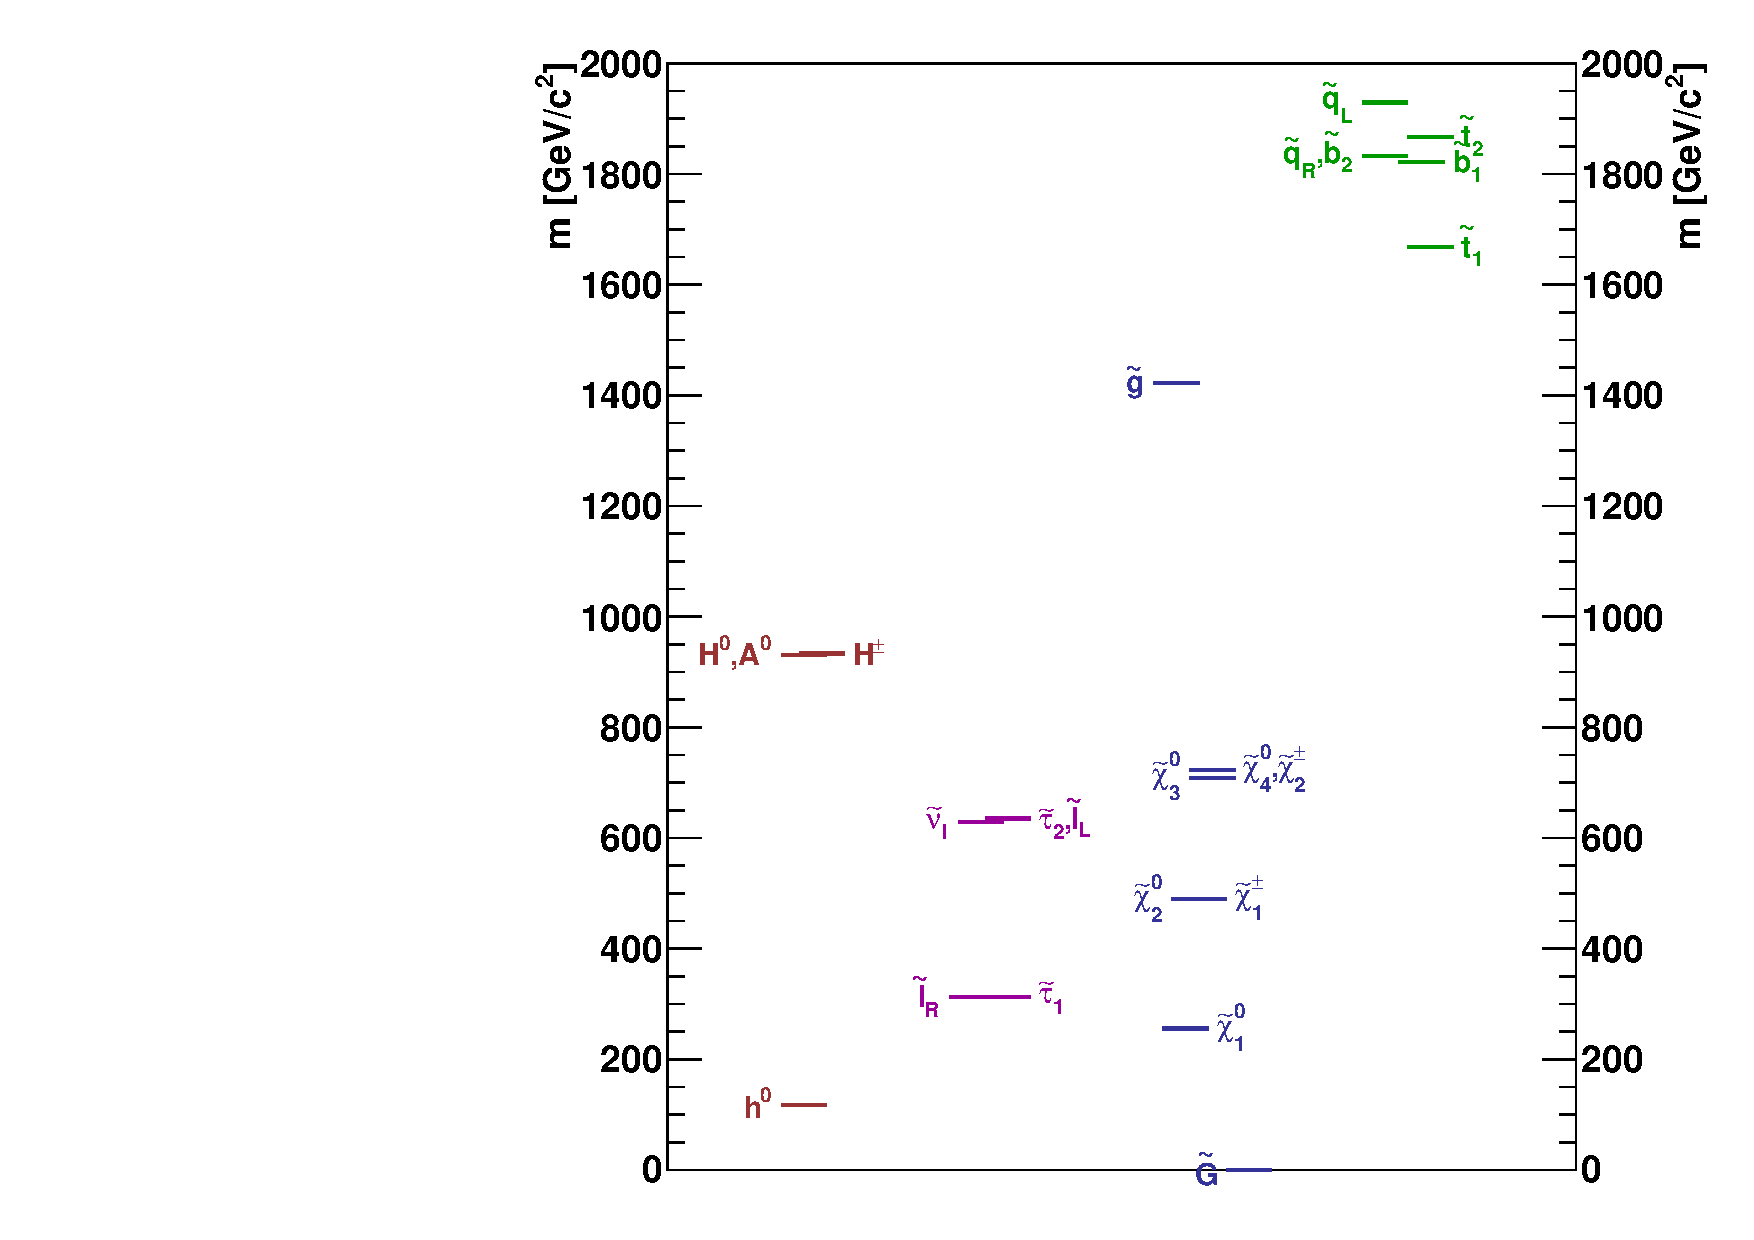
\includegraphics[height= 0.6\textwidth, width=0.7\textwidth]{THESISPLOTS/gmsb_Lambda180_CTau10000.pdf}  
%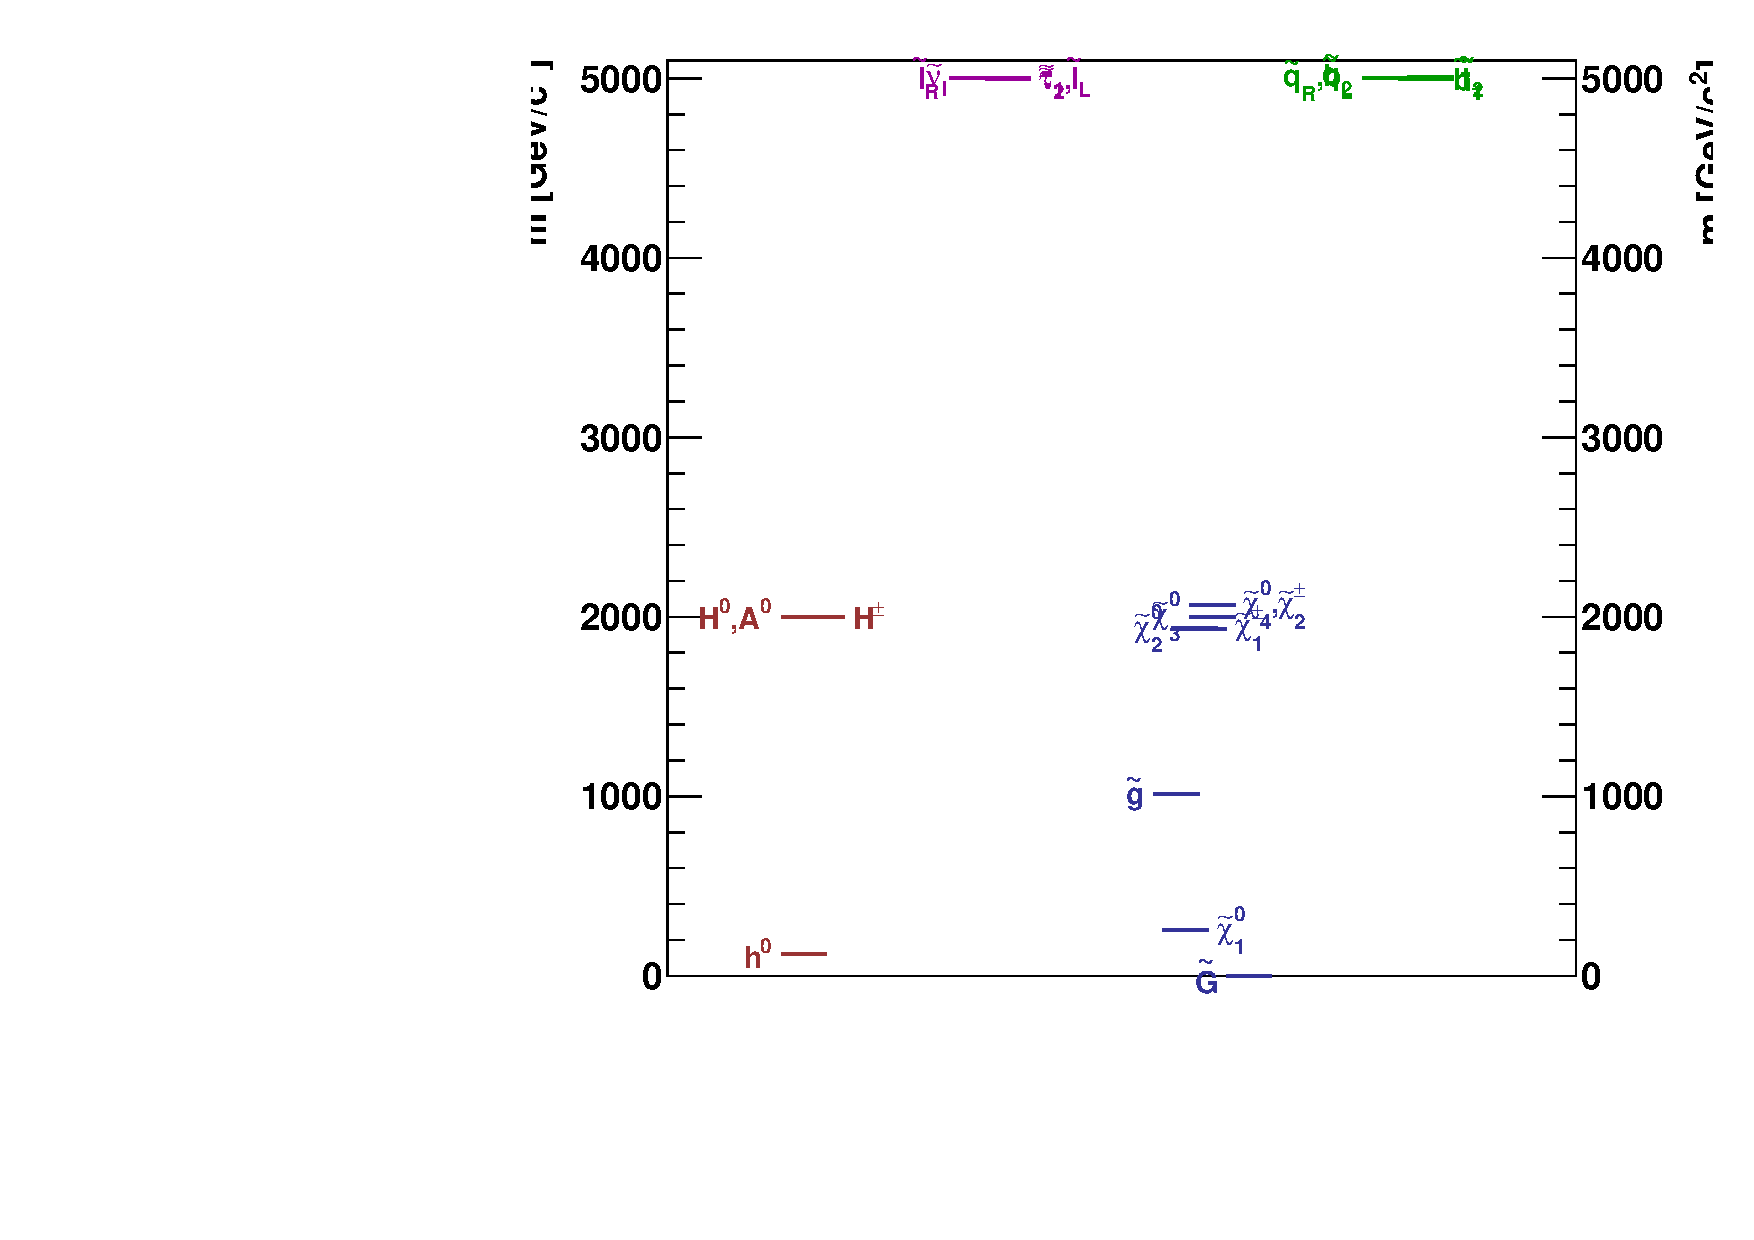
\includegraphics[height=2.5in]{THESISPLOTS/M3_1015_M1_255.pdf} }
\captionof{figure}{Supersymmetry particle mass spectra in the SPS8 or minimal GMSB~(mGMSB)model.}
%~(left) and GGM Model~(right) with mass of gluino ($M_{\tilde{g}} = 1.0$~ TeV)}
\label{fig:spectra}
\end{center}

In summary, MSSM predicts the existence of new particles whose spin~($S$) differ from their SM counterparts by half-integer. Bosons~(fermions) in the SM have superpartners which are fermions~(bosons).
The superpartners of SM fermions are scalars called \textit{sfermions}~($\tilde{l}$), sneutrinos~($\tilde{\nu}$) and squarks~($\tilde{q}$) while \textit{gluinos}~{$\tilde{g}$) are the superpartners of the massless gauge bosons of strong interaction, gluons. The scalar Higgs~(2 needed) bosons and the vector gauge bosons of Electro-Weak interaction have fermionic superpartners called \textit{higgsinos}, \textit{Winos} and \textit{Binos}. These can mix to form a pair of mass eigenstates called \textit{charginos}~($\tilde{\chi}^{\pm}_{j}, j=1,2$), \ie,
$\tilde{\chi}^{\pm}_{1,2}$ are mixtures of $\tilde{W}^{+}, \tilde{W}^{-}, \tilde{H}^{+}, \tilde{H}^{-} $ and a quartet of mass  eigenstates called \textit{neutralinos}~($\tilde{\chi}^{0}_{i}, i=1,...,4$), \ie, $\tilde{\chi}^{0}_{1-4}$ are mixtures of $\tilde{B}^{\circ}, \tilde{W}^{\circ}, \tilde{h}^{\circ}, \tilde{H}^{\circ} $.

%\paragraph{General Model}
%\paragraph*{•}
%Constructing a SUSY model requires that the model has gauge group describing the nature of particle interaction, a superpotential, and since the SUSY prediction of equal masses of boson and fermions is not observable, one must provide explicitly the method for spontaneously breaking supersymmetry. We have in the MSSM scenario seen the gauge groups to be exactly those of the SM, the superpontential with soft terms, however, we are yet to understand how supersymmetry is broken. SUSY breaking means that we find the lowest energy state for which the vacuum expectation values of the  SUSY generators $\mathrm{Q}_{\alpha} \ket 0 \neq 0$ or $\bar{\mathrm{Q}}_{\alpha}\ket 0 \neq 0$. Since one can always express the Hamiltonian of the system, $\mathrm{H}$ in terms of the SUSY generators, SUSY breaking can also be equally expressed as $\mathrm{H}\ket 0 \neq 0$. Neglecting spacetime-dependent effects and condensates, SUSY breaking is equivallently expressed as $\mathrm{V}\ket 0 \neq 0$, where $\mathrm{V}$ is the standard superpontential expressed in terms of the $\mathrm{F}$ and $\mathrm{D}$ terms. Thus, spontaneously breaking SUSY is equivalent to finding superpotentials for which neither $\mathrm{F}$ nor $\mathrm{D}$ terms simultaneously vanish in the lowest energy state. Suoerpotentials with non vanishing $\mathrm{F}$ terms are called  \textit{O'Raifeartaigh} or $\mathrm{F}$-term SUSY breaking models while those with nonvanishing $\mathrm{D}$ terms are called \textit{Fayet-Illiopoulus} or $\mathrm{D}$-term SUSY breaking models. Since in GMSB models, it is the $\mathrm{F}$ term which has a non-vanishing lowest energy state expectation value or vacuum expectation, this thesis only considers  \textit{O'Raifeartaigh} SUSY breaking models.
%\newline
%In GMSB models, this superpotential is termed the \textit{Hidden Sector}~(hidden because it couples only indirectly and very weakly to our "observable sector" of SM particles and their superpartners) and it is its dynamics which spontaneously breaks supersymmetry. The nature of this breaking is not relevant for phenomenology but rather the "\textit{mediators}" which communicate the effects of this breaking to the superpartners of the SM particles. Therefore, these mediators or agents must couple to this "Hidden Sector" as well as the "observable sector".
%This \textit{Messenger fields} in GMSB, have the usual SM gauge interactions  and through loops couple with the SM superpartners. As a result MSSM particles~(gauginos and sfermions) obtain SUSY breaking masses referred to as \textit{soft terms} through loop level interactions. This procedure allows for the observed mass and energy scale hierarchy is maintained. The mass of these messenger fields, $\displaystyle{\mathrm{M}_{\mbox{mess}}}$, along with $\left\langle\mathrm{F}\right\rangle$  defines the energy scale at which supersymmetry breaking is felt at the MSSM energy scale. If $\displaystyle{\mathrm{M}_{mess} \ll \mathrm{M}_{\mbox{Planck}}}$, $\mathrm{M}_{\mbox{Planck}} \approx 10^{19}$\GeV, then supersymmetry breaking occurs at a much lower energy scale instead at the Planck energy scale where gravitational interactions become very significant and the effects of the breaking is first felt by these Messenger fields and later communicated to the observable sector through SM gauge interactions.
%In terms of energy scales, the picture is such that spontaneous supersymmetry breaking occurs at an energy scale, $\left\langle\mathrm{F}\right\rangle$ which we denote as $\mathbf{F}$, for simplicity. This energy scale defines the mass, as seen in equation \ref{eq:GMass}, of the \textit{gravitino} which is the supersymmetric partner of gravity mediating particle, the \textit{graviton}. The gravitino has the same quantum number as the Nambu-Goldstone particle, the massless neutral Weyl fermion, the \textit{goldstino}, originating from supersymmetry breaking. 
%\begin{equation}{\label{eq:GMass}}
% m_{3/2} = C_{grav}\cdot\frac{\mathbf{F_{s}}}{{\sqrt{3}\mathrm{M}_{Pl}}}
%\end{equation}
%where $\displaystyle{\mathrm{M}_{Pl} = 1.3 \times 10^{19}}$~GeV.

%In GMSB models, the energy scale for which supersymmetry breaking is transmitted to the Hidden sector, $\mathbf{F}_{s}$ might not be the same as the original or fundamental sypersymmetry breaking energy scale, $\mathbf{F}$. If $\displaystyle{\mathbf{F}_{s} < \mathbf{F}}$ then the interaction between the hidden sector and the fundamental SUSY breaking is weak interaction and if $\displaystyle{\mathbf{F}_{s} \approx \mathbf{F}}$ and the interaction is strong.  It is necessary that this interaction is weak, as in this case GMSB models do not surfer from flavor violating interactions which are not observed in nature.
%The induced SUSY breaking scale in the hidden sector ${\mathrm{F}}_{S}$ and the mass of the messenger particles  defines the mass spectrum of the particles in the MSSM sector.
%The consequences of this is that one would no longer expect the mass of the gravitino $m_{3/2}$ to be given as in equation \ref{eq:GMass} but rather suppressed by $\mathrm{M}_{\mbox{mess}}/\mathrm{M}_{Pl}$ in GMSB models. In this mass spectrum scenario, the gravitino mass can be varied to a very small value only bounded by cosmological results, thus making it the lightest supersymmetric particle~(LSP). Spanning the gravitino mass is expressed as a fundamental parameter in GMSB modles, $C_{grav}$ which directly determines the lifetime of the next-to-lightest supersymmetry sparticle  decaying to the gravitino. We will see more of this ahead. Thus the parameters $\mathbf{F}_{s}$ and  $\mathrm{M}_{\mbox{mess}}$, determines the masses of the gauginos and sfermions of the MSSB in GMSB models.
%\newline
%A minimal GMSB model is one where the messenger sector consists of chiral supermultiplets of leptons and quark with the same quantum numbers $SU(3)_{C}\times SU(2)_{L}\times U(1)_{Y}$ as the SM gauge groups. That is, the messenger fields belong to some $SU(5)$ gauge group. The representations of these messengers fields are given in equation \ref{eq:MESS}.
%\begin{align}{\label{eq:MESS}}
%\tilde{\ell} \sim (1,2,1) \quad \tilde{\ell^{\prime}} \sim (1, 2^{\star}, -1) \\
%\tilde{q} \sim (3,1,-\frac{2}{3}) \quad \tilde{q}^{\prime} \sim (3^{\star}, 1, \frac{2}{3} )
%\end{align}
%These messenger fields, via a superpotential as in equation \ref{eq:WMESS} of a gauge singlet chiral supermultiplet $\mathrm{S}$, couple with an $\mathrm{F}$-term as in the O'Raifeartaigh model \cite{SM}. 
%\begin{equation}{\label{eq:WMESS}}
%W_{\mbox{mess}} = \lambda_{\ell}\mathrm{S}\tilde{q}\tilde{q}^{\prime} + \lambda_{q}\mathrm{S}\tilde{\ell}\tilde{\ell^{\prime}}
%\end{equation}
%We thus obtain SUSY breaking by allowing vacuum expectation values~(VEV) for both $\mathrm{S}$ and its auxiliary component $\mathrm{F}$ term as $\left\langle \mathrm{S} \right\rangle$ and $\left\langle \mathrm{F}_{s} \right\rangle = \mathbf{F}_{s}$, where the $\mathbf{F}_{s}$ does not have to coincided with $\mathbf{F}$ as mentioned earlier. The parameter representing this non equivalence,$C_{grav}$ is defined as shown in equation \ref{eq:CGRAV}. It is one of the fundamental parameters in GMSB models responsible for the lifetime of NLSP particle.
%\begin{equation}{\label{eq:CGRAV}}
%\mathbf{F} = C_{grav}\cdot\mathbf{F}_{s}
%\end{equation}
%This equation indicates that the non-zero VEV for the $\mathrm{F}$ term is responsible for fundamental SUSY breaking which is transferred to the messenger particles through radiative interactions as $C_{grav}$ is a dimensionless parameter.
%Leptons and fermions masses(\ref{eq:MMass}) of the messenger particles together with their scalar superpartners are obtained from diagonalizing the mass matrix.
%\begin{align}{\label{eq:MMass}}
%m^{2}_{\tilde{\ell}\tilde{\ell^{\prime}}} &= |\lambda_{\ell}\left\langle \mathrm{S} \right\rangle|^{2}, \quad \quad  m^{2}_{\tilde{\ell}_{\mbox{scalars}}} = |\lambda_{\ell}\left\langle \mathrm{S} \right\rangle|^{2} \pm |\lambda_{\ell}\left\langle \mathrm{F_{s}} \right\rangle |
%\\
%m^{2}_{\tilde{q}\tilde{q^{\prime}}} &= |\lambda_{q}\left\langle \mathrm{S} \right\rangle|^{2}, \quad \quad  m^{2}_{\tilde{q}_{\mbox{scalars}}} = |\lambda_{q}\left\langle \mathrm{S} \right\rangle|^{2} \pm |\lambda_{q}\left\langle \mathrm{F_{s}} \right\rangle |
%\end{align}
%By observing equation \ref{eq:MMass}, a general energy scale, $\mathbf{M}_{\mbox{mess}}$, for messenger particle's masses which is also an additional fundamental parameter in GMSB models can be defined as shown in equation \ref{eq:Mmess}.
%\begin{equation}{\label{eq:Mmess}}
%\mathbf{M}_{\mbox{mess}} = (\lambda_{q},\lambda_{\ell}) \left\langle \mathrm{S} \right\rangle 
%\end{equation}

%A common assumption in GMSB models according to~\cite{GMSB, SUSYBOOK} is that $\lambda_{q} \simeq \lambda_{\ell} \simeq \lambda $ and so $\mathbf{M}_{\mbox{mess}} = \lambda \left\langle \mathrm{S} \right\rangle$. However, in  Pure gauge mediated SUSY breaking models~(PGGM), $\lambda_{q} \neq \lambda_{\ell}$ \cite{PGGM}.
%In the MSSM sector, gauginos and scalars obtained their mass through one-loop and two-loop level interactions respectively given according to equation \ref{eq:MSSMMasses}.
%\begin{align}{\label{eq:MSSMMasses}}
%\mathbf{M}_{a} &= \frac{\alpha_{a}}{4\pi}\mathrm{N_{5}}\mathbf{\Lambda} \\ 
%\mathbf{m}^{2}_{\phi_{i}} &= 2\mathbf{\Lambda}^{2}\mathrm{N_{5}}\sum_{a=1}^{3}C_{a}(i) ( \frac{\alpha_{a}}{4\pi})^{2}
%\end{align}
%where $C_{a}(i)$ are constants of $\mathsf{O}(1)$, $\alpha_{a}$ are coupling constants and 
%\begin{equation}{\label{eq:Lambda}}
%\mathbf{\Lambda} = \frac{\mathbf{F}_{s}}{\lambda \left\langle \mathrm{S} \right\rangle } = \frac{\mathbf{F}_{s}}{\mathbf{M}_{\mbox{mess}}}
%\end{equation} 
%$\mathrm{N_{5}}$ is an additional parameter in GMSB models, specifying the number of messenger vector-like supermultiplets transforming under $SU(5)$. A motivation for $SU(5)$ is for the unification of gauge couplings at the GUT energy scale($M_{GUT} \approx 10^{16}$~GeV which is one of the major predictions of supersymmetry in unifying fundamental forces.
%$\mathrm{N_{5}}$ is chosen to be not very large so as to avoid gauge couplings diverging before GUT scale. In the minimal GMSB models such as the SPS8 benchmark working point model $\mathrm{N_{5}} = 1$.
%A simple diagrams for these corrections can be seen in figure \ref{fig:figMass}.

%\begin{figure}[ht]{\label{figMass}
%\begin{minipage}[b]{0.45\linewidth}
%\centering
%\includegraphics[height=7cm, width=\textwidth]{OneLoop_Gaugino_Mass.png}
%\caption{$c\tau_{\chi^{0}_{1}}$[mm]}
%\label{fig:1-loop level contributions from messenger particles giving rise to MSSM gaugino mass. The dashed(single) lines are messenger scalars(fermions).}
%\end{minipage}
%\hspace{0.5cm}
%\begin{minipage}[b]{0.45\linewidth}
%\centering
%\includegraphics[height=7cm,width=\textwidth]{TwoLoop_MSSM_Scalar_Masses.png}
%\caption{$Boost_{\chi^{0}_{1}}$ }
%\label{fig:2-loop level contributions from messenger particles giving rise to MSSM gaugino mass. The dashed(single) lines are messenger scalars(fermions) while the wavy lines are SM gauge bosons}
%\end{minipage}
%\end{figure}


%On the other hand in PGGM models~(\cite{PGGM}), gauge and scalar particles have separate mass definitions~(eqn:\ref{eq:MPGGM}) since $\lambda_{q} \neq \lambda_{\ell}$.
%\begin{align}{\label{eq:MPGGM}}
%\mathbf{\Lambda}_{G} &= \frac{\mathrm{F}_{s}}{\lambda_{q} \left\langle \mathrm{S} \right\rangle } \\
%\mathbf{\Lambda}_{S} &= \frac{\mathrm{F}_{s}}{\lambda_{\ell} \left\langle \mathrm{S} \right\rangle } 
%\end{align}

%$\mathbf{\Lambda}$ is the energy scale defining SUSY breaking at the MSSM level. It is known as the \textit{effective supersymmetry breaking scale} and determines the mass spectrum of gauginos and scalars in the MSSM.
%$\mathbf{\Lambda}$ as defined in equation \ref{eq:Lambda} is considered to be a model parameter in GMSB models especially in minimal GMSB modles like the SPS8 bench mark model.

%It is important to not that GGM models, \cite{GGM, GGM1, GGM2,MDINE1,MDINE2}, the mass of the gauginos $\mathbf{M}_{a}, a = 1,2,3$ defines the parameter space for these models.
%Using equation \ref{eq:CGRAV}, the fundamental SUSY breaking scale $\mathbf{F}$ can be redefined in terms of the effective SUSY breaking scale $\mathbf{\Lambda}$  and the Messenger particle mass scale $\mathbf{M}_{\mbox{mess}}$:
%\begin{align}{\label{eq:scale}}
%\mathbf{F} = C_{grav}\cdot \mathbf{\Lambda}\cdot\mathbf{M}_{\mbox{mess}} 
%\end{align}
%and from equation \ref{eq:GMass}, the gravitino mass is re-written shown in equation \ref{eq:GMass2}
%\begin{align}{\label{eq:GMass2}}
%m_{\tilde{G}} & = C_{grav}\cdot \frac{\mathbf{\Lambda}\mathbf{M}_{\mbox{mess}}}{\sqrt{3}\mathrm{M}_{pl}}
%\end{align}

%In summary, the parameters $\mathbf{\Lambda}$, $\mathrm{N_{5}}$, and  $C_{grav}$  determines the phenomenology of GMSB models.The gravitino can become very light with its mass bounded only by cosmological observations and as such is identified as  the least stable supersymmetry particle~(LSP). By changing the value of $C_{grav}$, which is equivalent to scaling the induced supersymmetry breaking energy scale, allowing for weak interactions between the hidden sector and the messenger particles, the mass of the gravitino, $m_{\tilde{G}}$, is changed. This influences the decay rate and lifetime of the next-to-lightest supersymmetry particle~(NLSP) decaying to the gravitino which can vary from being an instantaneous or prompt decay to being a long-lived particle decay.

%%%%%%%%%%%%%%%%%%%%%%%%%%%%%%%%%%%%%
\section{Gauge Mediated Supersymmetry Breaking Models}
%%%%%%%%%%%%%%%%%%%%%%%%%%%%%%%%%%%%%%%%%%%%%%%%%%
GMSB models have $5$ main parameters:
\begin{equation}{\label{eq:mGMSB}}
\left\{ \mathbf{\Lambda}, \quad \mathbf{M}_{\mbox{mess}},\quad \mathbf{N}_{5}, \quad \tan(\beta), \quad sgn(\mu),\quad C_{grav}\right\}
\end{equation}
where $\mathbf{\Lambda}$ is the effective supersymmetry breaking scale, $\mathbf{M}_{\mbox{mess}}$ is the mass of the messenger particle
involved in mediating supersymmetry breaking to the MSSM energy scale, $\mathbf{N}_{5}$ is the number of messenger particles.
The other parameters, $\tan\beta$ and $sgn(\mu)$ are related to the two Higgs bosons necessary for supersymmetry breaking with $\tan\beta$ being the ratio of the vacuum expectations values for both Higgs bosons. The sign of the Higgs potential is defined by
$sgn(\mu)$.
In these models, the gravitino can become very light with its mass bounded only by cosmological observations and as such is identified as  the Least Stable supersymmetric particle~(LSP).
The mass of the gravitino is expressed in terms of the parameter $C_{grav} $ according to equation \ref{eq:GRAV}.
\begin{align}{\label{eq:GRAV}}
m_{\tilde{G}} & = C_{grav}\cdot \frac{\mathbf{\Lambda}\mathbf{M}_{\mbox{mess}}}{\sqrt{3}\mathrm{M}_{pl}}
\end{align}
where $\mathrm{M}_{Pl} = 1.3 \times 10^{19}$~\GeVcc.
$C_{grav}$ is a scaling parameter, which determines the lifetime of the Next-to-Lightest-Supersymmetric Particle~(NLSP) 
since the neutralino decay rate to the gravitino will depend on the mass difference between the neutralino and gravitino.
\subsection{Phenomenology}
%\paragraph*{•}
Light gravitinos with unique gravitino-scalar-chiral fermion and gravitino-gaugino-gauge boson interactions shown in Figure \ref{fig:feynman_grav} in GMSB models allow for the gravitino mass to be as low as a few eV and up to an upper bounded for them to
provide the right amount of dark matter observed in the early universe. In addition to this, being neutral and stable makes them an excellent candidate particle for dark matter.
\begin{center}
\centering
\mbox{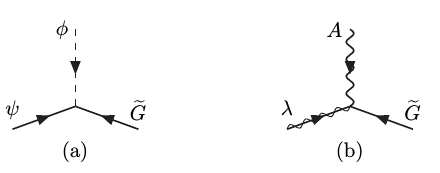
\includegraphics[height=0.3\textwidth, width=0.5\textwidth]{THESISPLOTS/Gravitino-GauginoCoupling.png}} 
%\quad \quad
%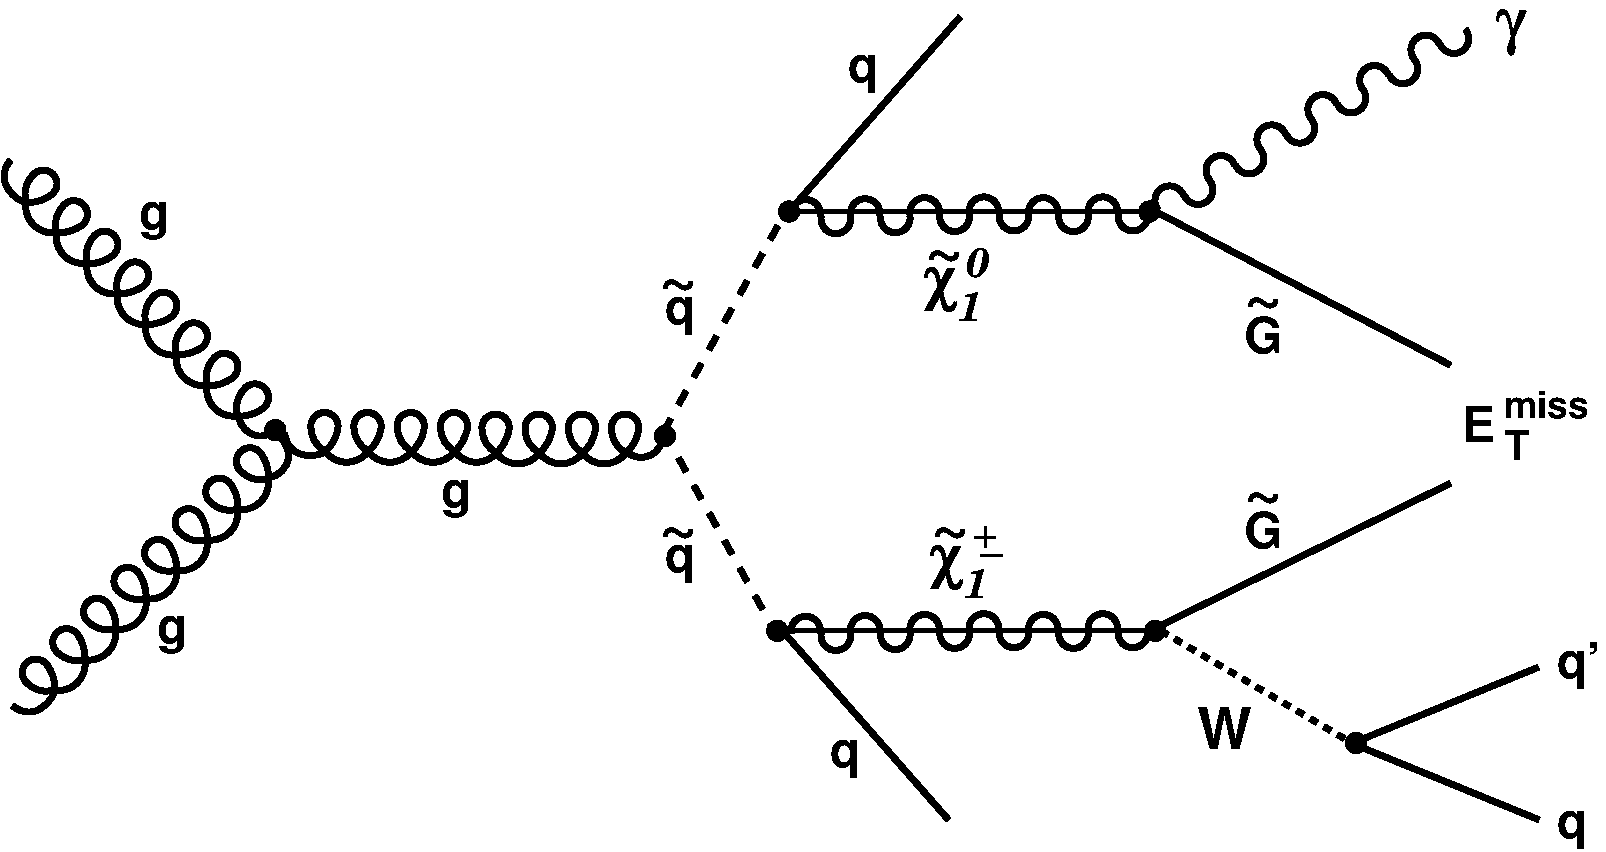
\includegraphics[height=0.3\textwidth, width=0.4\textwidth]{THESISPLOTS/SinglePhoton_squark.pdf}}
\captionof{figure}{Feynman diagrams of gravitino/golstino, $\tilde{G}$, gaugino and scalar interactions with superpartner pairs $(\psi, \phi)$scalar~(a)  and $(\lambda, \mathrm{A})$ gaugino~(b) decay to gravitino.}
\label{fig:feynman_grav}
\end{center}
%These light gravitinos with weak gravitino-gaugino or gravitino-scalar interactions allows for the decay of any next-to-lightest MSSM particle to a gravitino. 
%This decay rate depends on the mass of the gravitino $m_{\tilde{G}}$ as long as R-parity is conserved. Thus, in the decay of every MSSM particle, the gravitino will likely or eventually be included in its final states. We can  parametrised this decay rate by using $C_{grav}$. It is easy to see that $C_{grav} \geq 1$. It is important to note that there are other GMSB phenomenological observations which do not entirely considered the gravitino as the lightest supersymmetric particle.
%Thus in order to study the phenomenology of GMSB models, one can define a parameter space using the following parameters given in equation \ref{eq:mGMSB}. 
%\begin{equation}{\label{eq:mGMSB}}
%\left\{ \mathbf{\Lambda}, \quad \mathbf{M}_{\mbox{mess}},\quad \mathbf{N}_{5}, \quad \tan(\beta), \quad sgn(\mu),\quad C_{grav}\right\}
%\end{equation}
%These sets of parameters given in equation \ref{eq:mGMSB} are those we will be studying  within the minimal GMSB~(mGMSB).
% In other gauge mediating supersymmetry models like the General Gauge Mediation SUSY breaking~(GGM), $\left\{M_{3}(\mbox{gluino mass}), M_{2}(\mbox{Wino mass}), M_{1}(\mbox{Bino mass}),\tan(\beta), sgn(\mu), c\tau_{NLSP}\right\}$
%is the parameter space,\cite{GGM1,GGM2}.
%In GGM models, colored sparticles are not required to be heavier than their Electro-Weak sparticles allowing for greater discovery potential at hadron collider\cite{DSHIH}. Thus, allowing for possibility of many candidates NLSP particles and not only the neutralino as in the case with mGMSB models like the SPS8 model.
%For Pure General Gauge Mediation SUSY breaking~(PGGM), the parameter space is rather scan using $\displaystyle{\left\{\Lambda_{G},\Lambda_{S}, \mathrm{M}_{\mbox{mess}}\right\} }$ parameter set.
%Of all other possible decay modes in GMSB models, this thesis is interested only in decays where eventually, the Next-To-Lightest SUSY particle~(NLSP) decays to the lightest SUSY particle~(LSP) which is the gravitino and its SM partner; i.e if particle, $\tilde{p}$ is the NLSP, then it will decay is given according to equation \ref{eq:NLSPDECAY}.
%\begin{equation}
%%\tilde{p}\rightarrow p + \tilde{G}
%\end{equation}
The decay of the NLSP to the gravitino is always accompanied by the SM partner of the NLSP, in order to conserve R-parity.
If the particle, $\tilde{p}$, is the NLSP, its decay to gravitino and its SM particle, $p$, is given as $ \tilde{p}\rightarrow p + \tilde{G}$.
In the SPS8 benchmark model, the choice of parameters is as follows: $\mathbf{M}_{\mbox{mess}} = 2\mathbf{\Lambda}$, $ \tan(\beta)=15$, $\mathbf{N}_{5}=1$. Only $\mathbf{\Lambda}$ and $C_{grav}$ are allowed to vary, \cite{SPS8}.
The gravitino~($\tilde{G}$), is the LSP. The NLSP, $\tilde{p}$, is the lightest neutralino~($\tilde{\chi}^{0}_{1}$). 
There are four types of neutralinos which are a mixture of the supersymmetric particles Bino~($\tilde{B}^{\circ}$),  Wino~($\tilde{W}^{\circ}$), higgsino~($\tilde{H}^{\circ}_{u},\tilde{H}^{\circ}_{d}$), depending on the choice of parameters  $\Lambda$, $\tan\beta$, and $sgn(\mu)$.
The particle $p$ could be a photon~($\gamma$), Z boson~$(Z)$ (or $Z^{\prime}$) and a higgs boson~($h$).
This thesis, for experimental convenience, will focus on the parameter space for which the particle $p$ is a photon~($\gamma$) and $C_{grav} > 1$.
This ensures that the lifetime of the NLSP is long enough but still its decay happens within the detector volume and the resulting photon is delayed or non-prompt on length scales of size of the detector.
The decay rate for a NLSP to its SM partner and a gravitino can be approximated using only the mass of the
NLSP and the effective supersymmetry breaking scale, $\mathbf{F} = C_{grav}\cdot \mathbf{\Lambda}\cdot\mathbf{M}_{\mbox{mess}}$
giving in equation \ref{eq:drate}.
%(More details can be found in \cite{SM, GMSB, NLSP}).
\begin{equation}{\label{eq:drate}}
\Gamma(\tilde{NLSP} \rightarrow \gamma\tilde{G}) \approx  \frac{m^{5}_{\tilde{NLSP}}}{\mathbf{F}^{4}}
\end{equation}
This approximation is almost the same for the non-minimal GMSB models except that additional parameters are present showing explicit dependence of the neutralino life time on its states as a mixture of other supersymmetric particles.
%It is important to observe here that, the decay rate is large for smaller values of the fundamental SUSY breaking scale or equivalently smaller gravitino mass for a fixed neutralino mass. Thus if $m_{NLSP}$ is of the $\mathrm{O}(100$~\GeV) or more and $\sqrt{\mathbf{F}} \ll 1000$~\TeV, meaning $m_{\tilde{G}} \leq 1$~\KeV, then the above decay rate is of the order than can be observed at hadron collider detectors.
%%%%%%%%%%%%%%%%%%%%%%%%%%%%%%%%%%%%%%%
%%%%%%%%%%%%%%%%%%%%%%%%%%%%%%%%%%%%%%%%
\subsection{Long-Lived Particles in GMSB Models}\label{long-lived}
%\paragraph*{}
%In addition to mass, charge and spin being experimental handles use in the search for new physics, a 
Measuring a particle's life time or distance traveled before it decays can be a useful method to uncover new fundamental interactions.
As the lifetime is related to the decay rate which is determine by the particles interactions and available energy space.
%Since through life time measurements, one has direct access to measuring and understanding and in some cases excluding the energy scale and fundamental parameters involved in a new interaction.
\subsubsection{Production of supersymmetric particles at Hadron Colliders}
%%%%%%%%%%%%%%%%%%%%%%%%%%%%%%%%%%%%%%%%%%%%%%%%%%%%%%%%%%%%
The production of a particle in a particle collider is a probabilistic process.
This probability is expressed as a measurable quantity called \textit{cross section}. For example,
the cross section of producing a particle in proton-proton collider such as the LHC, is the probability 
that the proton beams will collide and interact in a certain way to produce that particle. Although this
cross section~($\sigma$) is measured in units of area as \textit{barns}~($1b = 10^{-24}~\cm^{2}$), usually it has 
very little relation to the physical interpretation of area as used in everyday life. It is rather a technical
term for counting the number of the particle produced when these proton beams collide.
The cross section of producing the particle depends on the available energy of the 
proton beams compared to the mass of the particle, the type of interaction 
during collision which in turn depends on the coupling constants, and the flux of the proton beams.
The rate or number per unit time of the particle produced at a specific particle collider is
given as a product of its cross section times the instantaneous luminosity~($\mathscr{L}$).
The instantaneous luminosity is the number of incident particles per unit area per unit time.
The typical cross section of producing a supersymmetry particle at the LHC is of the order of $1~pb =10^{-12}\times 10^{-24}~\cm^{2}$ or at times $1~fb = 10^{-15}\times 10^{-24}~\cm^{2}$ for extremely rare SUSY processes. While that for a standard model process like the production of the $\PZ$ or $\PWpm$ bosons is of the order of a few $nb = 10^{-9}\times 10^{-24}~\cm^{2}$.
This means there are more SM processes than supersymmetry process and so the search for supersymmetric particles in the LHC  is very challenging.
% since most SUSY production cross-section are very small compared to an overwhelming high cross-section processes from the standard model.

The rate of production of a supersymmetric particle at the LHC depends on the mass of supersymmetric particle. 
The masses of supersymmetric particles are much higher than those of SM particles and as a result, the cross section for producing supersymmetry particles at a hadron collider is much smaller compared to that for SM particles.
%This probability depends on the distribution of type of incoming particles inside the colliding protons with enough proton energy fraction to create a supersymmetric particle. Since the mass of the supersymmetric particle being create depends on the available center of mass energy of the colliding partons. In a hadron collider like the LHC, gluons are the one of these partons with the highest probability of proton energy fraction distribution. Sea quarks such as up and down quarks which make up the proton as well as valence quark which can exist inside the proton provide their energy fraction is large enough can also collide to create SUSY particles. The figure \eqref{PDFs} show the parton distribution function against its energy fraction on the horizontal axis within a proton. The probability of creating a SUSY particle depends on the momentum transfer $Q$ of these partons.
The cross section of a given supersymmetric process  happening at the particle collider can be computed and compared with experimental measurements. Using diagrammatic representations called \textit{Feynmann} diagrams of the process happening, the cross section is derived from the Feynmann diagrams as the computed probability of the process.
Supersymmetry processes which leads to the production and decay of neutralino~($\PSneutralinoOne$) at the LHC can involve electro-weak and strong interactions. 
The production of supersymmetry particles in strong interactions have larger cross sections compared to electro-weak processes because of the strong coupling in strong interaction processes. Many interaction processes in the LHC are strong interactions as the LHC is a proton-proton collider.
We show in Figure \ref{fig:SUSYPROD} a diagram showing the variation of the supersymmetry production cross section against the mass of the supersymmetric particle. From this figure, it is clear that the production of supersymmetric particle at the LHC through strong interactions like $pp \rightarrow \PSgluino\PSgluino, \PSq\PSq$ is higher than through electro-weak interactions like $pp \rightarrow \PScharginopm\PScharginomp, \PSneutralino\PScharginopm$. 
\begin{center}
\mbox{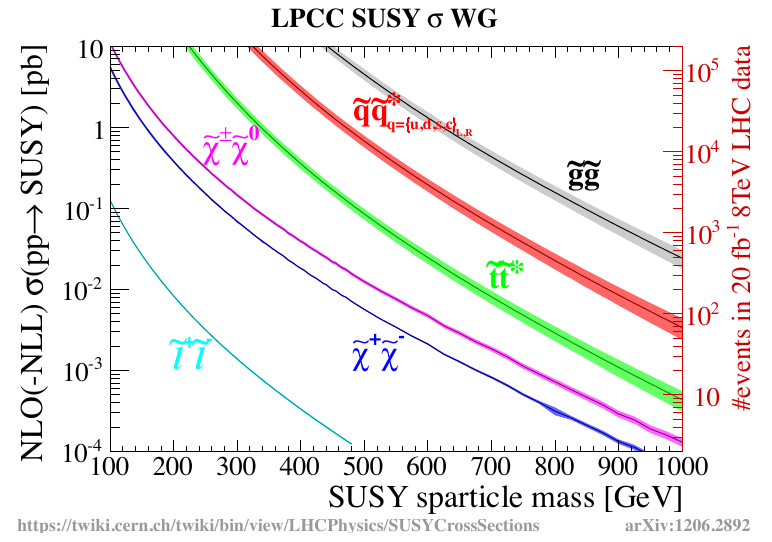
\includegraphics[height=0.7\textwidth,width=0.7\textwidth]{THESISPLOTS/SUSY_Xsec.png}}
%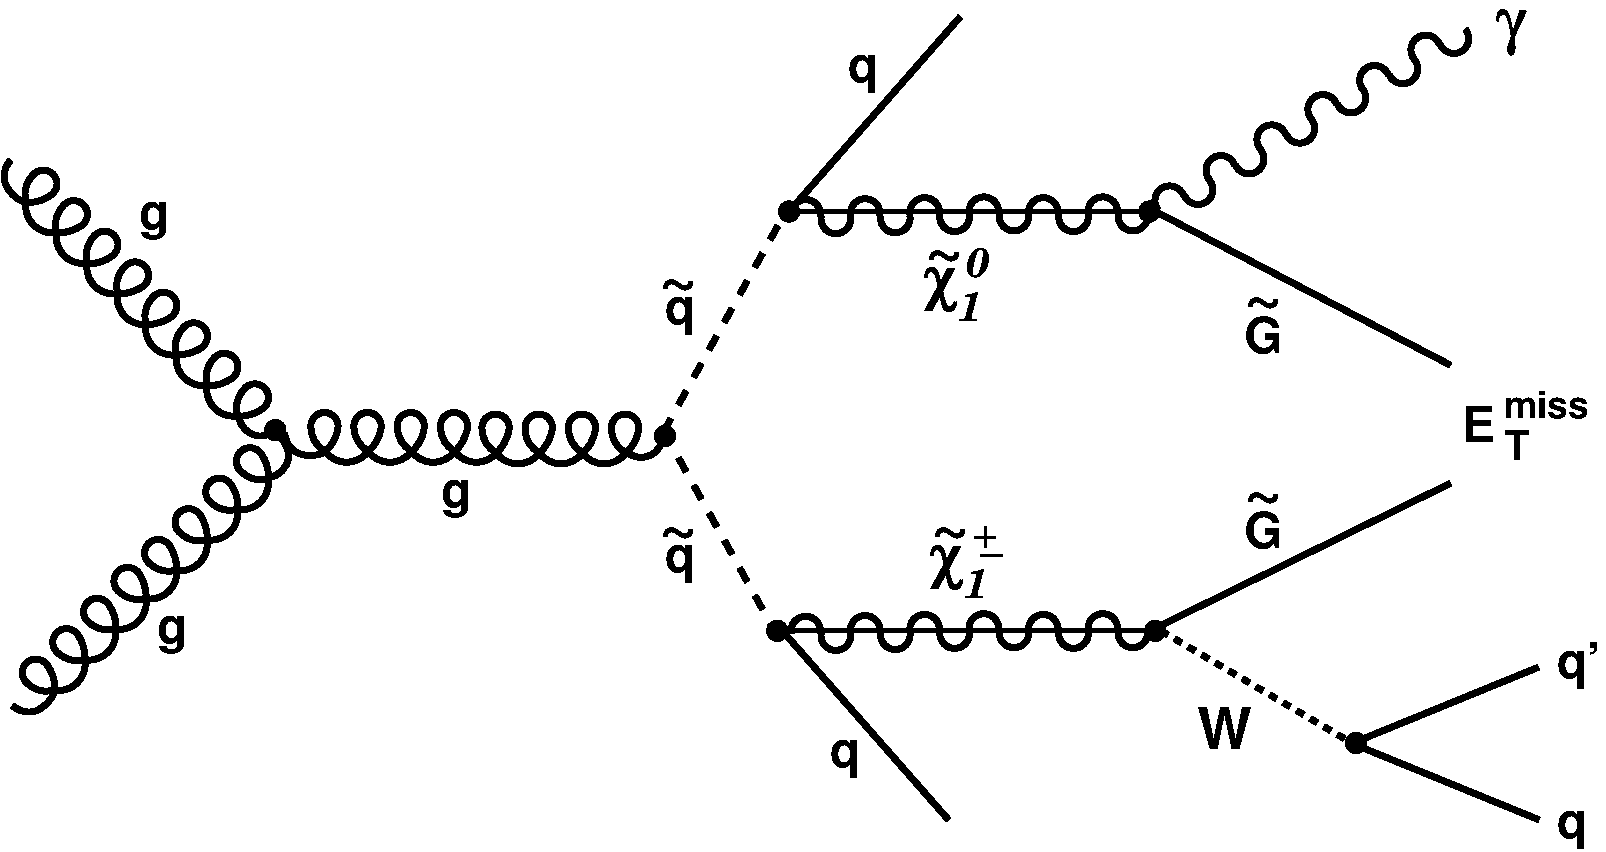
\includegraphics[width=2.5in]{THESISPLOTS/SinglePhoton_squark.pdf}} \\
\captionof{figure}{Supersymmetry production cross-section against sparticle mass for different modes of supersymmetry production at a proton-proton collider. $pp \rightarrow \PSgluino\PSgluino$ processes have the dominant production cross section.}
\label{fig:SUSYPROD}
\end{center}
%The production of neutralinos through Electro-Weak interactions are known as \textit{direct} production of neutralinos while those due to strong interactions which is the dominant mode of supersymmetry production at the LHC, 
We will concentrate on the production of neutralinos from processes like $pp \rightarrow \PSgluino\PSgluino, \Psquark\Psquark$, as these processes have a higher production cross section at the LHC.
We mentioned earlier that a probable manner in which neutralinos can be produced is from the production and subsequent decay of higher massive supersymmetric particles. Some of these higher massive supersymmetric particles include squarks~($\PSq$), excited squarks~($\PSq^{\star}$) and gluinos~($\PSgluino$). In this scenario, the neutralino is produced \textit{indirectly} or as we say from the \textit{cascade decay} of higher massive supersymmetric particles.
The Feynmann diagram for these production processes, $pp \rightarrow \PSgluino\PSgluino$, $\PSq\PSq^{\star}$, are given in figure \ref{fig:feynman_gsDiag}. Squarks and gluinos do not directly decay into gravitinos but through neutralinos and eventually to gravitinos because their coupling to the gravitinos is not possible. The reason for this is that, in GMSB models, there are no gravitino-gluino-gauge boson or gravitino-squark-gauge boson couplings but rather gravitino-gaugino-gauge boson or gravitino-scalar-chiral fermion couplings. 
\clearpage
\begin{center}
\centering
\mbox{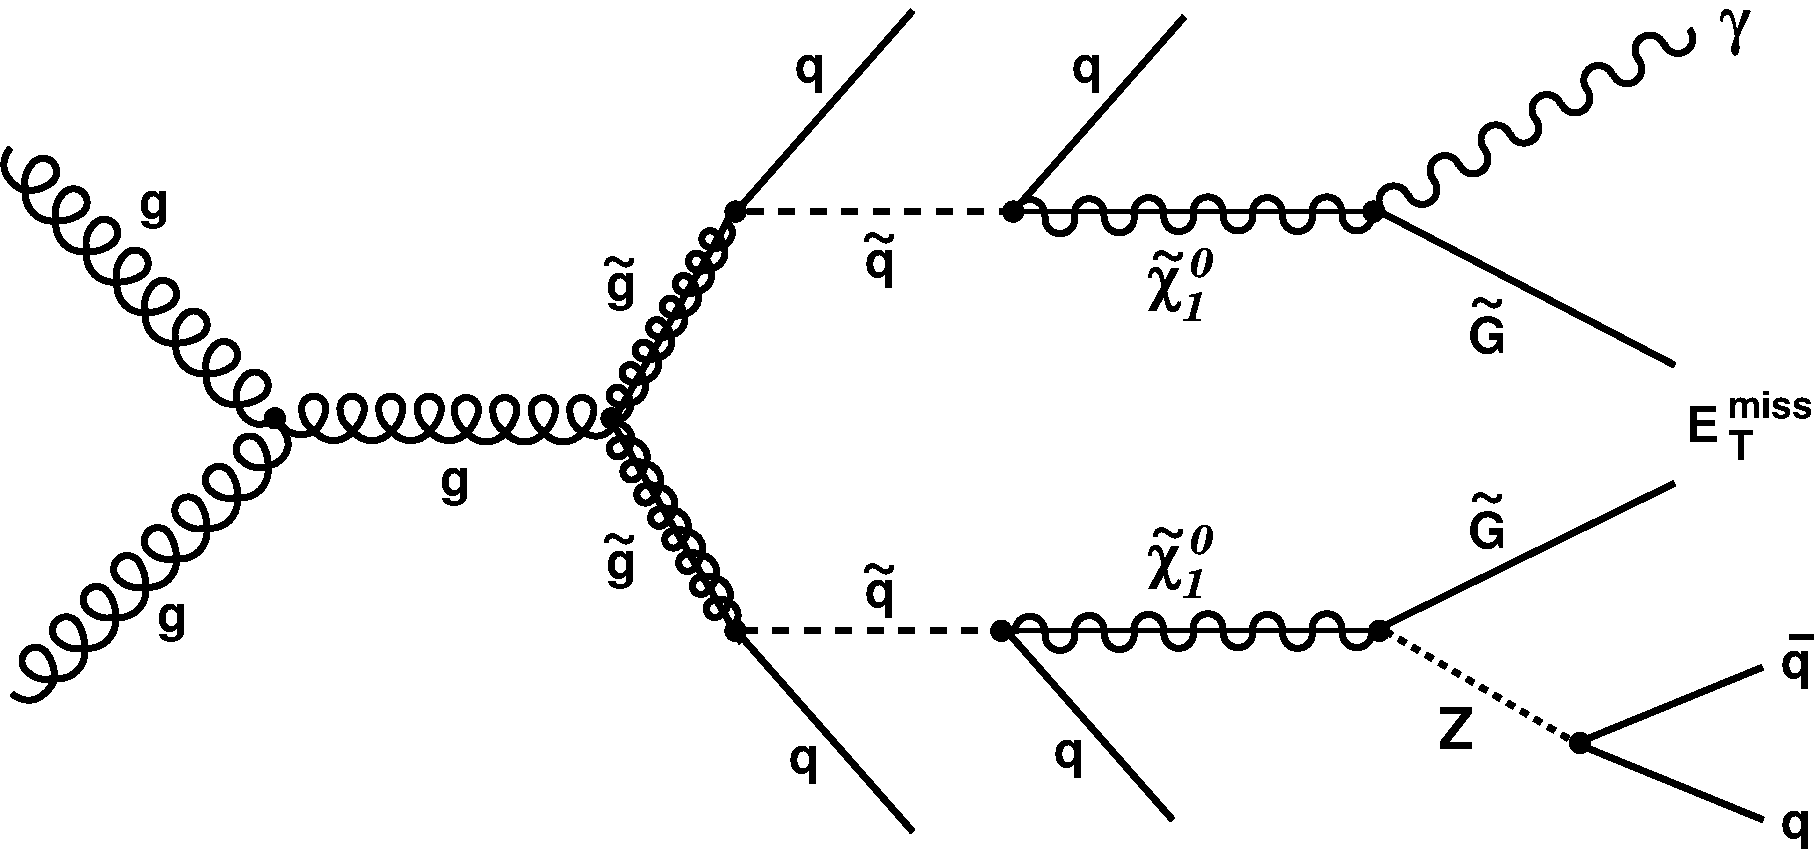
\includegraphics[height=0.27\textwidth, width=0.4\textwidth]{THESISPLOTS/SinglePhoton_gluino.pdf} \quad \quad
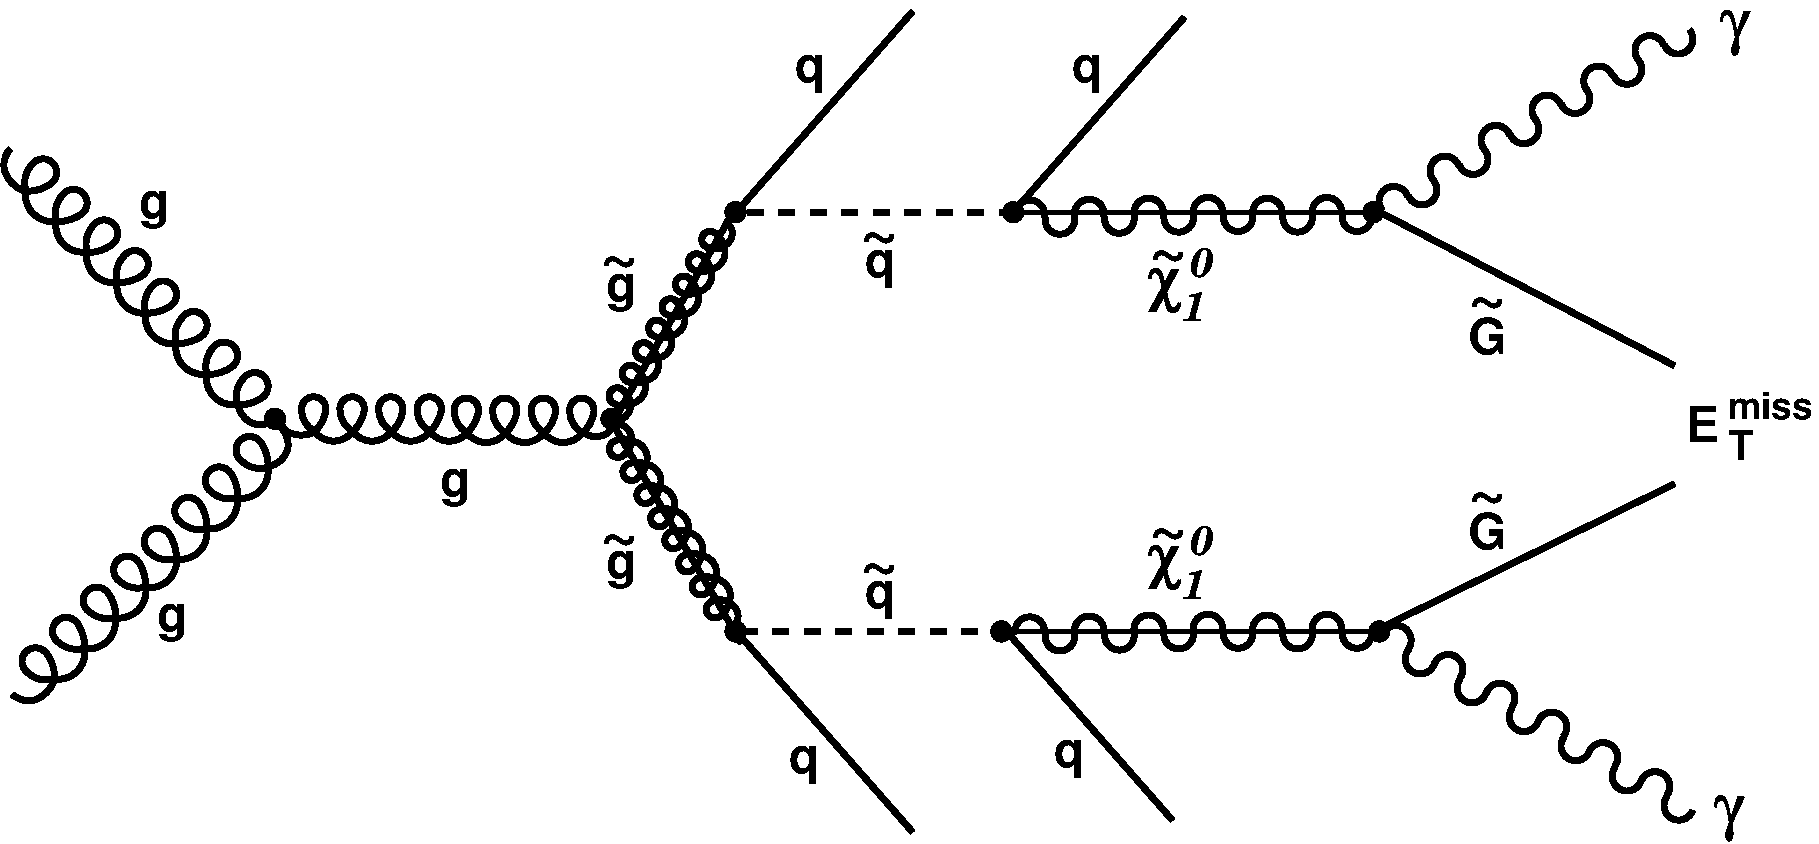
\includegraphics[height=0.27\textwidth, width=0.4\textwidth]{THESISPLOTS/Diphoton_gluino.pdf}} \\
\hspace{0.5cm}
\mbox{   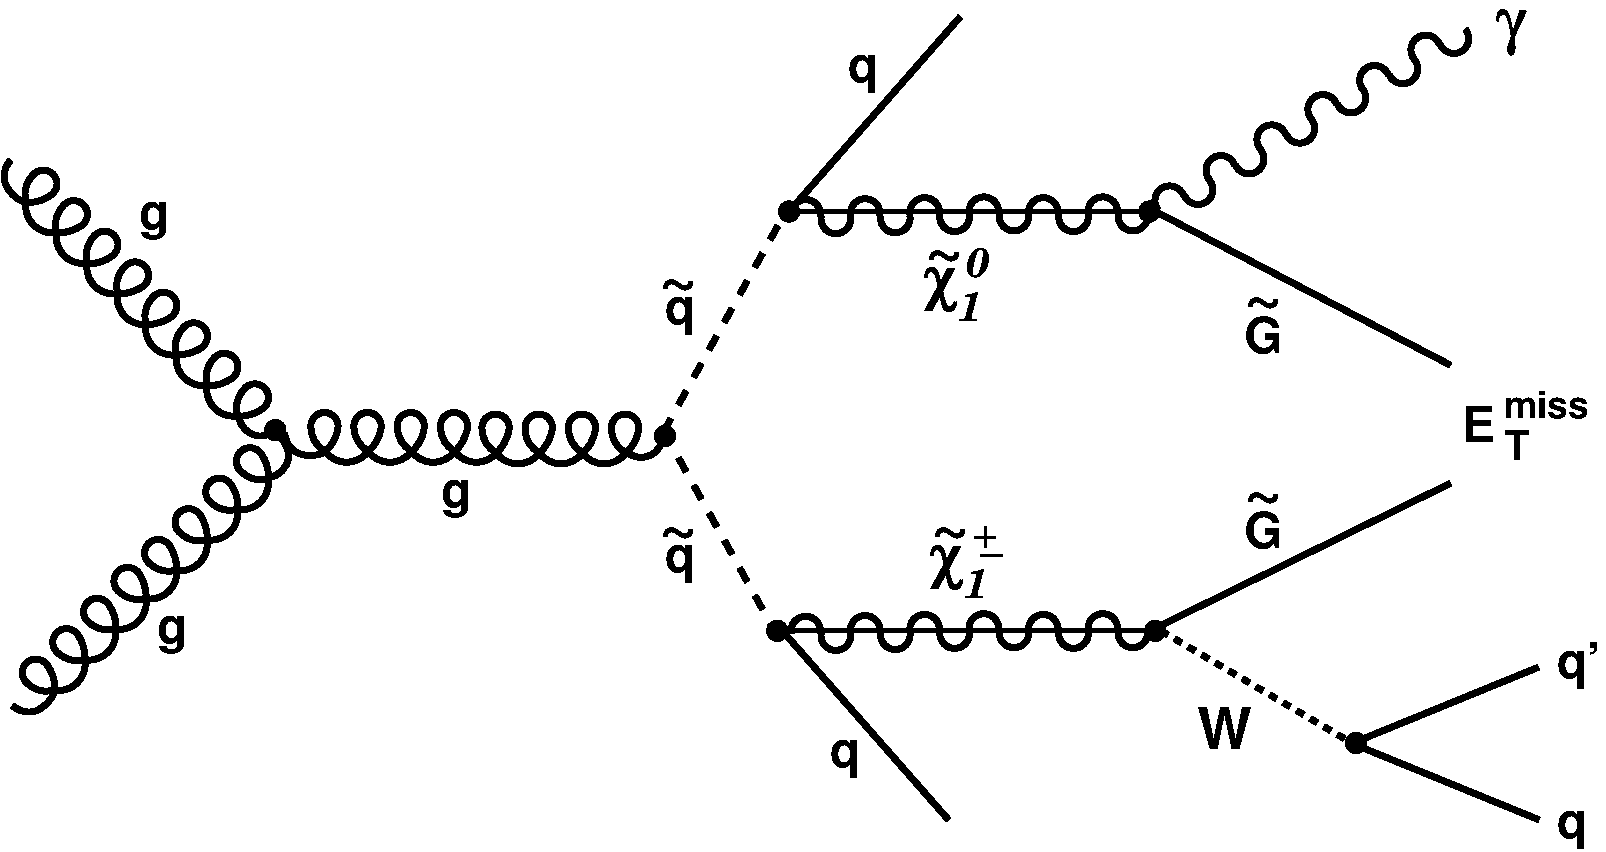
\includegraphics[height=0.25\textwidth, width=0.4\textwidth]{THESISPLOTS/SinglePhoton_squark.pdf}\quad \quad
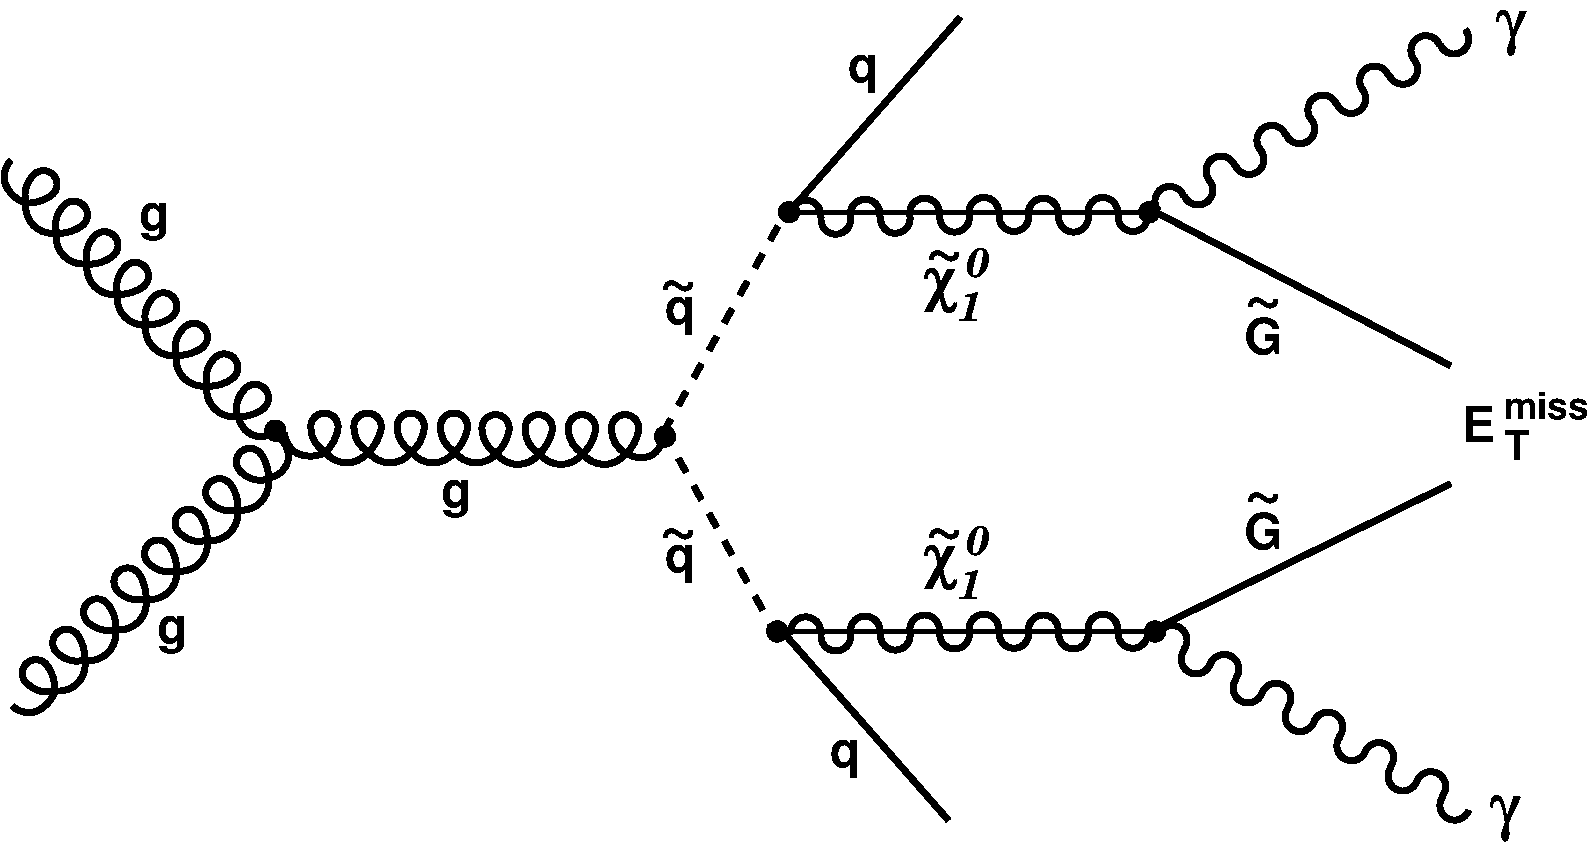
\includegraphics[height=0.25\textwidth, width=0.4\textwidth]{THESISPLOTS/Diphoton_squark.pdf} }
\captionof{figure}{Feynmann diagrams for neutralino production from the cascade decay of a produced gluino~(\textit{top}) and squark~(\textit{bottom}).
The final event has a single~(\textit{left diagrams}) or double photons~(\textit{right diagrams}) neutralino decay at LHC.}
\label{fig:feynman_gsDiag}
\end{center}
%The list of feynman diagrams presented for SUSY processes in figure \ref{fig:feynman_gsDiag} is not exhaustive. As previously mentioned, SUSY production cross-sections are very small compared to SM production processes. A production cross section is express in term of a unit called a \textit{barns}~(b). ($1~b = 10^{-28}$~$m^{2}$). Because this number is quite small it is usually further express with suffix in front of the unit barn such as \textit{nano}~(n) or \textit{pico}~(p) or \textit{femto}~(f).
%%%%%%%% DECAY %%%% LONG-LIVED%%%%%%%
\subsubsection{Particle Decay Rate}
When a particle is produced, say particle $\mathbf{A}$, its coupling to other particles, say particles
 $\mathbf{B_{1}}\cdots \mathbf{B_{n}}$, where $n$ is total number of particles particle, 
allows for it to decay into these other particles. 
In addition to the coupling, if the mass of particle $\mathbf{A}$ is greater than
the total sum of mass of particles $\mathbf{B_{1}}\cdots \mathbf{B_{n}}$, i.e $m_{\mathbf{A}} > m_{\mathbf{B_{1}}} + \cdots 
+ m_{\mathbf{B_{n}}}$, then we say, particle $\mathbf{A}$ \textit{decays} to particles $\mathbf{B_{1}}\cdots \mathbf{B_{n}}$.
Particle for which no such channel for decay is possible are termed \textit{stable}. Our current understanding is that
only the electron~($\Pe$) and the proton~($\Pproton$) are stable( although there are theories which predict the
proton to decay after $10^{34}$ years and also theories where stable heavy or light particles 
will explain the nature of Dark Matter. This time through which a particle lived before
it decays is called its \textit{lifetime}. Particle decays in which the particle decays instantly as soon as they are produced
are called \textit{prompt} decays while particle decays with observable lifetime are \textit{non-prompt} decays.
Non-prompt decays might range from factors of a seconds \ie \textit{nanoseconds}~($1$~ns $= 10^{-9}$~s) to minutes.
%Particles which live long enough to travel distanced comparable to the detector size(of the order of a few minutes) are equally referred to as \textit{long-live} particles.  
%Almost all particles disintegrate or \textit{decay}, most very rapidly. Collectively particles which disintegrate are said to be unstable while the few which do not are said to be stable. Those which take a long time to disintegrate are termed meta-stable or "\textit{long-lived}" particles. The length of the decay time and context will tell whether a particle is meta-stable or long-lived. The stability of a given particle is measured with respect to the age of the universe~(13.7 billion years). The only understood stable particles in nature are the \textsf{electron}(and \textsf{anti-electron})~($e$), \textsf{up}~($u$) and \textsf{down}~($d$) quarks and their anti-quarks, the \textit{photon}~($\gamma$), the lightest \text{neutrino}~($\nu_{e}$) and the \textit{graviton}. 
%Particles decay by transforming from one type of particle or generation unto another either through interactions, radiation or oscillation.  This decay, in analogous to our everyday experience depends on the their interaction strength with possible particles they can decay into. For example, strongly interacting particles will decay almost immediately while weakly interacting particles will naturally take some time. However, this is not the whole story, as quantum effects will also determine the particles nature of decay.
%which is understood to be about 13.7 billion years old. 
%Meta-stable particles which are composite~(bound states of elementary particles), are more unstable and easily decay into particles with smaller mass. An example of a meta-stable particle is the \textit{neutron}~(\textsf{$udd$}) which on its own, outside the atomic nucleus can remain stable for about 15 or so minutes. While, neutrons living inside some atomic neuclei can live for a period of time comparable to the age of the universe. Another meta-stable particle like the proton~(\textsf{$uud$}) seem very stable but can possibly decay after a very long period of time. It is speculated that the proton can remain stable for up to a period of about $10^{33}$ years. Atomic nuclei can also be considered as meta-stable living for about a tiny fraction of a second. Thus for all practical purposes, the proton is considered a stable particle while the neutron is considered a \textit{long-lived} particle.  It is believed that if \textit{dark matter} is made of particles then those particles  must be very, very, very long-lived with time also comparable  to or beyond  the age of the universe.
%Particle disintegration is understood as the interaction between a given particle and its daughter particle(s). This interaction could be electromagnetic, weak, strong, any pair or maybe all three types of interactions. 
%The stability of a particle is determined by the properties of the particle combined with  conservation laws of a quantum number or conserved quantity like energy, spin, momentum, angular momentum and charge. Other factors may also play an important role such as phase space~(availability of lighter particles to decay into), violation of some fundamental property like \textit{strangeness} or the mediating particle usually a boson being very massive compared to the momentum transfer between the parent and the daughter particle. These laws combined with particle's properties leads to a set of rules which are (almost) entirely determine whether a particle can decay or not or at most decay very rarely.  
%These set of rules can be summarized as follows:
%\begin{itemize}
%\item All particles must and should decay to two or more particles.
%\item The mass of the decaying~(parent) particle must exceed the sum of the mass  of the particles produced~(daughter particles) in its decay.
%\item There must be charge conservation i.e, the total electric charge of the parent particle must equal or match the total electric charge of the daughter particles.
%\item The total number of fermions or spin-1/2 particle before and after the decay must change only by an \textit{even} number.
%\item The total number of quarks minus the total number of anti-quarks must not change in any decay.
%\item The nature of of interaction and degree of phase space available must all be satisfied in order for any decay to take place.
%\end{itemize}
In particle decay, strong \textit{couplings} and large \textit{mass difference} between the parent and the daughter particle(s) leads to faster the decay. The process of obtaining the decay rate during experiments is expressed mathematically as; $N(t) = N(0)e^{-t/\tau}$, where both $N(t)$ and $N(0)$ are the number of the particles present at time $t$ and at the beginning, $t=0$. $\tau$ is the particle's \textit{lifetime}.
\newline
The rate at which a particle decays is its \textit{decay width}~(\textbf{$\Gamma$}).
The decay width relies on the availability of daughter particle(s) the parent particle can couple to and the mass(es) of the
daughter particle(s) must be less than the mass of the parent particle. Thus, a given particle, $\mathbf{A}$
will preferentially decay to particles  $\mathbf{C_{1}}\cdots \mathbf{C_{n}}$ with which it has stronger couplings and its mass is much larger than their masses. This preferential decay into a specific set of particles or channel brings about terms like \textit{Branching Ratio}~(BR). The BR is related to the total decay width through $BR =\Gamma/ \mathbf{\Gamma_{Total}}$, where,  $\mathbf{\Gamma_{Total}}$ is the particle's total decay width and $\Gamma$ is its decay width to a preferential channel.
% It is an experimentally measurable quantity which can also be computed in theory. A particle's decay rate $\Gamma$ can depend on the strength of a given interaction involved in the decay.As such the experimental measurement of decay rate provides access towards understanding the type of interaction involved and important parameters governing the underlying interaction or mediating particles involved in a given decay. Thus, measuring a particle's decay rate can be used as a direct access to search for other interactions beyond the known interaction and thus provide evidence for new physics. 
The decay width is related to lifetime, $\tau$, as the inverse of the lifetime. This relationship is expressed as given in Equation  \ref{eq:RATE}.
\begin{equation}{\label{eq:RATE}}
  \tau = \frac{\hbar}{\Gamma}
\end{equation}
$\tau$ is the particle's lifetime in a frame where the particle is not moving.
It is convenient to express lifetime in units of lengths rather than time.
The lifetime in units of lengths \eg meters~(\m), is $c\tau$, where $c$ is the speed of light in vacuum. $c\tau$ is also called the \textit{proper decay length} just as the lifetime, $\tau$, is also called the \textit{proper lifetime}.
Since most particles have mass and travel with velocity $\vec{v}$ not equal to $c$,
this distance travel considering $|\vec{v}| \neq c$ is fully expressed using equation \ref{eq:DECAY}.
\begin{equation}{\label{eq:DECAY}}
 \vec{L} = \vec{\beta} \gamma c\tau
\end{equation}
where $\vec{\beta} = \frac{\vec{v}}{c} $, $\vec{v}$ is the particle's traveling velocity and $\gamma = \frac{1}{\sqrt{1 - \frac{v^{2}}{c^{2}}}}$ is a factor relating the motion when it is not moving~(rest frame) to a frame where it is moving.
Equation \ref{eq:DECAY} can also be expressed in as $\vec{L} = \frac{\vec{p}}{m}c\tau$, in terms of the particle's momentum $p$ and mass, $m$. A particle with a large mass,$m$, produced with a small momentum, will travel slow covering some distance before it decays.
Since decay rate, $\Gamma$, depends on the coupling, particle decaying through electromagnetic, weak and strong interactions
have very different decay rates. Particles decaying through strong interactions 
have the largest decay rate and equally shortest lifetime of about $10^{-17}$ to $10^{-25}$~seconds. Electromagnetic particle decays have lifetime which can vary from $10^{-12}$ seconds to about $10^{-9}$ seconds and weak interactions have lifetimes that can vary from $nanoseconds$ to several minutes.
Particle lifetime may also vary from a few femtoseconds~(1~fs $1 = 10^{-15}$~s) to the age of the universe or equivalently 
its measured distance traveled can vary from a few $\mu$m to billions of km \cite{SM,SUSYBOOK}. 
%Terms to refer to each range in lifetime are unfortunately few.
The term \textit{long-lived} particles refers to particles which live long enough to travel a distance comparable to the detector size.
This distance traveled might range from a few $\mu$m to meters.

% Thus the decay length, $c\tau$  for electromagnetic interaction, can be very different to that of weak and strong interactions. The decay length for strong interactions is the shortest because of the strong nature~(coupling constant $\approx 1$) of strong interaction. The weak and electromagnetic interactions have much smaller coupling constants thus often leads to longer decay length. There are some exceptions to this due to other factors playing a key role than only the strength of a given interaction such as the size of the available phase space and the difference in mass between the parent and the sum of the mass of the daughter particles.
%The table and graph below show the mass and decay length of SM particles and their interaction.
%\begin{equation}
% TABLE SHOWING SM particle decay rates and interactions involed as well as mass Vs decay length.
%\end{equation}
%In particle physics experiments it is very challenging to measure the  life time or decay length or a particle  by measuring the time it travels from where it was produced to where it decayed. Rather, the number of events present initially and that observed after a time period t is used to measure the lifetime of a particle. The decay rate ( or life time) of a particle is related to the number of particles observed though the equation:
 %\begin{equation}
% N(t) = N_{0}\exp\left(\frac{-t}{\tau}\right) = N_{0}\exp\left(\frac{-\Gamma t}{\hbar}\right) 
 %\end{equation}
%where \textit{N(t)} is the number of particles observed at an arbitrary time \textit{t} and $N_{0}$ is the number of particles observed at an initial time where it is assumed no particle has decayed yet usually at $ t = 0 $.
%A distribution of the observed number of particles( usually a Poisson distribution) can be plotted with time measured. The resulting distribution if fitted with a Poisson distribution faction and the parameter of the Poisson distribution function extracted  to give us the decay rate or life time of a particle.
%\newline
%Particles with large decay length or long life time are commonly referred to as \textit{Long-Live}~(LL) particles. Many models beyond the SM predict the existence of such particle. They are also understood to be prime candidates for particles making up DM.
%Before we dive into such models, it is necessary to understand in detail the decay of particles and factors which determine a particle's decay length as well as the kind of LL particles considered detectable in a multi-particle physics detector such as those at the Large Hadron Collider~(LHC) CERN pursued in this thesis.
%\paragraph*{}
%Particles described by the SM come in different types of long-lived.  First, we have the stable elementary (as we currently believe) such as the electron and neutrinos. Second, we have the meta-stable elementary such as the muon and finally the (very) long-lived composite particles such as the neutrons and protons. By referring to the different classes of particles according to their life time, we can asked the question, what properties of a particle makes it stable, meta-stable or long-lived?
%\newline
%There are three possible answers to this question:
%\begin {itemize}
%\item A particle could be the lightest state carrying a conserved quantum number and as such remain entirely stable e.g the electron and proton.
%\item The decay of a particle to another lighter particle could only be  made possible through some suppressed or effective coupling and as a result ends up being meta-stable e.g the muon
%\item If the mass of a particle is relatively close in quantity to the particle it is decaying into such that their difference in mass is quite small, the decay will be eventually suppressed. This goes by the name lack of phase space for decay e.g decay of neutron ($ n \rightarrow p + e^{-} + \bar{\nu}_{e} $). In this scenario the difference in mass between the neutron (n) and the proton (p) is $\approx 1.293$ MeV and as a result determines the type of associated particle produced in this decay as observed.
%\end{itemize}

%long-lived particles in this thesis, we cover mostly \textit{massive neutral meta-stable} particles  referred here as \textsf{Neutral Massive Long-Lived Particles}~(NMLLP). These are either elementary or composite neutral particles with life-time within the detectable range of a collider detector i.e few nanoseconds. In general, 
%A rather more descriptive name would be Neutral Massive Meta-Stable Particles(NMMP) since these particles are not very long-lived in the real sense but might decay into other elementary particles which for all practical purposes can be observable at collider detectors.
%\newline
%We have restricted ourselves to electromagnetic (local U(1) gauge symmetry) neutral particles as their charge counterparts can be studied using conventional magnetic spectrometer and ionization methods as shown in this studies for Heavy Stable Charge Particles (HSCP).


%\subsection{Decay of supersymmetric particles in CMS detector}
\subsubsection*{Neutralino as Long-Lived Neutral Particle}\label{NeutralinoDecay}
The neutralino being the next-to-lightest-supersymmetry particle~(NLSP), can decay into a photon~(\Pphoton), Higgssino~(\PSHiggszero), \PZ boson and gravitino~($\tilde{G}$) \cite{NLSP, GMSB}.
% produced from the cascade decay of squarks and gluinos can decay into a gravitino and a gauge boson or scalar particle. This decay is also a probabilistic process and can be expressed and quantified as a single real number. 
% There are always many options for a given particle to decay into and each of these options is quantified by a number known as the \textit{Branching  Fraction} or \textit{Branching Ratio}. Summing all the branching ratios for all the different decay processes gives the total \textit{Decay Width}. The total decay width, can also be computed and expressed as a single real number in units of \GeV or \MeV (\GeV = giga electron volt $=10^{9}$~eV). 
 %In the case of the neutralino as the NLSP, the decay width depends on the nature of its interaction with the gravitino and an associated gauge boson or scalar field.
%\paragraph*{}
The probability for a neutralino~($\PSneutralinoOne$), produced with energy $\mathrm{E}_{\PSneutralinoOne}$ and mass $m_{\PSneutralinoOne}$ to travel a distance $x$ before decaying to a photon and gravitino in the laboratory frame can be expressed as 
$\displaystyle{\mathcal{P}(x) = 1 - \exp{\left(- \frac{x}{\mathrm{L}} \right)} }$, where the distance traveled in a particle detector by the neutralino is given by Equation \ref{eq:dl}.
\begin{equation}{\label{eq:dl}}
\displaystyle{\mathrm{L} = \left(c\tau_{\PSneutralinoOne}\right) \cdot {\left(\beta\gamma\right)}_{\PSneutralinoOne}}
\end{equation}

From Equation \ref{eq:dl}, it is clear that this distance depends on two main factors. The boost factor, $\left(\beta\gamma\right)_{\tilde{\chi}^{0}_{1}} = \frac{|\vec{p}_{\PSneutralinoOne}|}{m_{\PSneutralinoOne}} = \sqrt{\left(\frac{E_{\PSneutralinoOne}}{m_{\PSneutralinoOne}}\right)^{2} - 1}$, which indicates how fast the neutralino is traveling before it decays. 
For slow moving neutralino, $\left(\beta\gamma\right)_{\tilde{\chi}^{0}_{1}} \ll 1$. 
%For the case of the neutralino, $\beta$ can be redefined as given in equation \ref{eq:beta}.
%\begin{equation}{\label{eq:beta}}
%\displaystyle{\left(\beta\gamma\right)_{\tilde{\chi}^{0}_{1}} = \frac{|p|}{m} = \sqrt{\left(\frac{E}{m}\right)^{2} - 1} 
%\end{equation}
%Equation \ref{eq:beta} shows that in order for the condition $\beta \ll 1$ to be true, one would require
 
This means that the momentum~($p_{\PSneutralinoOne}$) of the neutralino during production from gluino or squarks decays must be much smaller than the its mass, $m_{\PSneutralinoOne}$. 
Neutralinos, produced, with their mass and momentum satisfying the slow condition, $p_{\PSneutralinoOne}/m_{\PSneutralinoOne} \ll 1$,  are definitely good candidates for detectable long-lived neutralinos. 
The other factor is the inherent long lifetime,$c\tau_{\PSneutralinoOne}$, of the neutralino. Neutralinos with
$c\tau_{\PSneutralinoOne} > 1$ are long-lived and would make good candidates for detectable long-lived neutralinos.
This inherent neutralino lifetime can be expressed as given in equation \ref{eq:ctau}. 
\begin{equation}{\label{eq:ctau}}
c\tau_{\PSneutralinoOne} \approx \left(\frac{m_{\tilde{\chi}^{0}_{1}}}{\mbox{ GeV}}\right)^{-5}\left(\frac{\sqrt{\mathbf{F}}}{\mbox{TeV}}\right)^{4}
\end{equation}
\begin{equation}{\label{eq:pdlength}}
c\tau_{\tilde{\chi}^{0}_{1}} \approx C^{2}_{grav} \left(\frac{m_{\PSneutralinoOne}}{\mbox{GeV}}\right)^{-5}\left(\frac{\sqrt{\mathbf{\Lambda}\cdot\mathbf{M}_{\mbox{mess}}}}{\mbox{TeV}}\right)^{4}
\end{equation}
It is important to note that by changing the supersymmetry breaking scale, $\mathbf{F}$, the lifetime of the neutralino also changes.
In the SPS8 model, the parameter $C_{grav}$ is used to adjust the inherent lifetime of the neutralino.
Thus, we re-write the neutralino lifetime as given in equation \ref{eq:pdlength}.
This equation is used to simulate physics events with the production and decay of neutralino in CMS detector using Monte Carlo~(MC) simulations. 
%\paragraph*{•}
The supersymmetry breaking scale, $\mathbf{\Lambda}$, determines the mass of gluino~($\PSgluino$), squarks~($\PSq$) which decay to
the neutralino. Therefore the neutralino momentum, $p_{\PSneutralinoOne}$ is determined by the masses of gluino and squarks.
If the gluino or squark decays to the neutralino in association with a many gluons and quarks seen in the detector as \textit{jets},
then the neutralino momentum is small with the ratio $p_{\PSneutralinoOne}/m_{\PSneutralinoOne} \ll 1$, this means the neutralino is slow and therefore long-lived. However, if the gluino or squark is decays with less number of jets, then the neutralino momentum is
not so small and the neutralino is not very long-lived.
It is worth nothing that kinematic properties of the neutralino like momentum, arrival time at the CMS ECAL and the number of associated jets can be influenced by the gluino or squark decay properties.
The gluino or squark is produced during proton-proton~($pp$) collisions at the LHC and the data recorded by the CMS detector is analyzed to search for events with neutralino decay.
%Since mass of SUSY particles like gluino, squarks and also neutralino is kept fixed by the SUSY effective breaking scale $\mathbf{\Lambda}$ as shown in equations \ref{eq:MSSMMasses}, the neutralino $\pt$ will depend o the number of associated quarks observed as \textit{jets} produced during the gluino or squark decay. Gluino or squark decays with very low jet multiplicity will lead to the production of large $\pt$ neutralinos which eventually leads to more boost factor while high jet multiplicity will lead to low $\pt$ neutralinos and hence low boost or $\beta$ factor. It is important to note that in either case, this depends also on the measured $\pt$ of the jets whether is low or high jet multiplicity cases. It is also worth mentioning that the photon produced from neutralino decay can also be arrived with large delayed time in situations where the photon arrival path to the detector is not a direct straight path but rather deviated as a result of a highly boosted neutralino produced from gluino or squark decay.

%In addition to the boost factor, the inherent proper decay length, $c\tau$,  will also determine the extend to which a long-lived neutralino is detectable at a particle detector. Neutralino with very long lifetime, $c\tau$, beyond the detectable length of the particle detector will obviously travel out of the detector before decay and as a result are often not detectable while neutralinos with very short lifetime may also be undetectable  as their decay length travel is not enough to be able to separate them for background events in a detector environment like the LHC unless other methods are employed like using its impact parameter distance travelled. However, this is only applicable in scenarios where the neutralino decays into a charged particle with tracks in the detector such that its decay production vertex can be used to correctly calculate and extracts the neutralino impact parameter or in other sophisticated detectors which the direction of the particle from neutralino decay is accessible. This the is case with ATLAS particle detector and not so with CMS detector.

%With $C_{grav}$, one could  one could change the decay length of the NLSP such that its decay occurs within the volume of the detector such that the resulting photon is delayed. This gives a unique signature for discovering SUSY in hadron colliders as photons produced from SM interactions are prompt.




%\begin{equation}\label{DRate}
%c\tau_{NLSP} = 9.9 \times 10^{-8}\frac{1}{k_{1\gamma}}\left(\frac{m_{NLSP}}{100 GeV}\right)^{-5}\left(\frac{\sqrt{\mathrm{F}}}{10TeV}\right)^{4}
%\end{equation}

%%%%%%%%%%%%%%%%%%%%%%%%%%%%%%%%%%%%%%
%\subsection{Why is the search for neutral long-lived particles important?}
%\paragraph*{}
% Finding answers to fundamental questions such as the following: What is the origin of neutrino masses, Why are there only 3 types of leptons and quarks? Where do all the parameters in SM come from? Other big questions include: What is Dark Matter ~(DM)? is DM made of particles? Can one detect these particles? Why is there so much asymmetry between matter and anti-matter in our universe? Is there some energy scale or early epoch in the evolution of the universe where all the fundamental forces behaved as a unique kind of force. Do baryons such as the proton exist forever? What is the lifetime of the proton? What is Dark Energy~(DE)? Is the Universe expanding indefinitely? Are there other Universes? 
% provide added impetus to search for particles BSM. We believe that the discovery of a long-live particle which are not known to exist within the current SM will provide unique access to understanding physics BSM and making measurements which can provide answers to most of the above questions.
%\newline{}
%These questions have been addressed in two major fronts: Theoretically which involves lots of model building and Experimentally which can be divided into Observational as well as Collider Experiments. Most of these experiments involves the search for w new physics phenomenon. In this Thesis, we have decided to address some of these questions by searching for New Physics phenomenon or New Particles ~(NP) in a Hadron Collider experiment. 
%As a consequence, there are many searches for New Particles or New Physics~(NP) 
%Searching for LL neutral particles decaying to photon using timing gives us a unique advantage compared to other experiments as we expect very limited background process contribution from SM. Most of our background will be detector originated contributions
%Infact, we are searching for some NP which have been predicted to exist in nature by many Theoretical extensions of the SM collectively referred to as Beyond the Standard Model~(BSM). We will describe one of such models in the next section below.
%We are interested in searching for neutral NP through their lifetime. 
%Infact, our search using lifetime gives us a wide range of search techniques  depending on the lifetime of the LL particle ranging from quantitative measurements to statistics. The figure below  shows the wide variety of techniques which can be used to search for LL particles in general.
%\begin{equation}
%\mbox{ADD figure of techniques for Searches using LL}
%\end{equation}
%\begin{figure}
%\centering
%\includegraphics[scale=0.5]{}
%\caption{Different techniques to Search for LL particles.}
%\end{figure}
%Using equations \eqref{ctau}, precise measurement of fundamental parameters in SUSY or new physics can be archived.
%Another advantage is that, the our search for neutral particles  is unique in that a lot of previous searches been performed for charged particles but very limited for neutral LL particles since DM is speculated to be made of stable neutral particle(s) with long lifetime, we might as well go for DM. 
%We also use lifetime because no particle with lifetime $\gtrsim10^{-7}$~s and mass $\gtrsim 1.5$~GeV has been found and obviously because our detector has a very good timing resolution as can be seen in the section of the CMS detector in this thesis.
%\newline{}
%There have been previous attempts to search for quasi-stable neutral massive particles but all the search results show no evidence for neutral particles with long lifetime.  
%or neutral particles in general or neutral hadrons in particular 
%The challenge with such an experiment is that neutral particles cannot be studied using conventional magnetic spectrometer as they are not affected by magnetic field because they are charge~(local 
%U(1) gauge symmetry) neutral.
%Nevertheless, there are countless theoretical as well as observational reasons why studying these particles using novel experimental techniques is very important in the field of particle physics. 
%Some of these reasons will emerge naturally as we see in the subsequent sections below.
%We will attempt to give our humble lists of reasons in the following
%sections why we believe it is fundamental to study these particles.
%\subsubsection{Theory Motivation.}
%Physics BSM can be summarized to answering three major theoretical questions:  Is there a reliable explanation  
%behind the ordering in mass of SM particles as observed? This is the Hierarchy problem.
%Is there a single theory which can provide a derivation for all the 
%numerous parameters (19) in the SM and also unify all the fundamental forces of nature? Grand Unified Theories (GUT). 
%What is DM and Dark Energy (DE)?
%(DE is the stuff that is responsible for the accelerated expansion of our universe).
%And finally being a particle physicist it is only natural to ask if DM is made up of particles and if yes,
%Can one construct a model which can consistently describe DM as is already the case with visible matter in SM?
%\newline
%Most of the efforts in the last decades in theoretical particle physics has been to find answers to the above questions.
%\subsubsection{Experiment and Observation Motivation }
%As early as 1956 Reines and Cowan\cite{Neutrino} observed that when a neutron decays into a proton and an electron, an elusive particle called neutrino is also produced. The observation of neutrinos was later incorporated into the SM. In the formulation of the SM, the neutrinos are considered massless.
%However, recent results from experiments \cite{NeutrinoMix} have shown that neutrinos of different flavours can oscillate or mix into one another. The only way they can do this is if they have a tiny but finite mass. Recent experiments measuring the different neutrino flavours and their mass difference point towards the existence of a much larger theory that can incorporate the existence of neutrino masses and the observed phenomenon of neutrino mixing in which the SM is embedded in it   and can be understood as a low energy version of a much broader and deeper theory.
%\paragraph*{}
%Galactic and supernovae observations using the Hubble and a host of other telescope as well as results from Baryonic Acoustic Oscillation~(BAO) and WMAP reveal unique matter content of our universe. In addition to these cosmological observations including galaxy profiles,cluster formation, large scale structure formation and Cosmic Microwave background~(CMB) power spectrum can be somehow explained by DM \cite{WMAP}. These observation reveals about 25\% of our universe is made of DM with the current DM relic density is measured to be  %${\POmega}_{DM}h^{2} = {0.105} ^{\p 0.021}_{\m 0.030}$
%However, the question of "What is DM?" remains a very interesting one to both the particle physics astronomy society.
%Understanding DM and the rest of our universe will be crucial for future developments in high energy physics from both theory and experimental fronts.  
%A possible property of DM is that they must be made of up long lived neutral particles. There are candidate particles from SUSY which have these properties. A few of these include lightest neutralino~(\PSneutralinoOne) and gravitino~($\tilde{G}$). From the GMSB point of view, because gravitinos are stable, neutral and very weakly interacting; they are seen as good candidates for the particles which make up DM. 
%\subsubsection{Current Experimental Limits}
%Past Experiments seems to indicate that the remaining un %searched phase space for possible existence of SUSY particles %in shrinking.
%%%%%%%%%%%%%%%%%%%%%%%%%%%%%%%%%%%%%%%%%%%%
%%%%%%%%%%%%%%%%%%%%%%%%%%%%%%%%%%%%%%%%%
%\subsection{Physics}
%\paragraph*{}
% The SM of particle physics in all its glory is the most precise and well developed model describing and providing our understanding of how energy, space and time interact with each other. We will begin by describing the current status of the SM highlighting areas where there could be need for further development in the format of questions.
%%%%%%%%%%%%%%%%%%%%%%%%%%%%%%%%%%%%%%%%%%%%%%%%%%%%%%%%%%%%%%%%%%%%%%%%%%%%%%%%
%%%%%%%%%%%%%%%%%%%%%%%%%%%%%%%%%%%%%%%%%%%%%%%%%%%%%%%%%%%%%%%%%%%%%%%%%%%%%%%%
\section{Previous Search Experiments} \label{PrevResults}
%%%%%%%%%%%%%%%%%%%%%%%%%%%%%%%%%%%%%%%
The have been previously other search experiments for neutral long-live particles decaying to photons. Obviously, negative findings  from these experiments led to possible search exclusion regions in terms of the lifetime, mass and cross section of the existence of supersymmetry particles in different supersymmetry models. Results from experiments(DO, CDF, CMS and ATLAS) \cite{LEP,CDF,ATLAS, CMS, ATLAS1} of the search for Neutralino NLSP decaying to photon and gravitino interpreted using the SPS8 benchmark model is
 shown in \ref{fig:UpperLimits}. These results show that within the SPS8 model, neutralinos with mass $m_{\PSneutralinoOne} \leq 245$~\GeV and proper decay length $c\tau_{\PSneutralinoOne} \leq 6000$~mm have not been found at hadron colliders.
 The diagram on the left of figure \ref{fig:UpperLimits} are exclusion results in the neutralino mass or
 supersymmetry breaking scale $\mathbf{\Lambda}$ on the horizontal axis and the nuetralino lifetime, $c\tau_{\PSneutralinoOne}$
 on the vertical exis from the $7$~TeV search analysis by the ATLAS experiment
 while the diagram on the right is that for CMS experiment. The colored regions on the plots shows the parameter space where
 these searches have been performed and the findings were negative.

%%%%%%%%%%%%%%%%%%%%%%%%%%%%%%%%%%%%%%%
\begin{center}
\centering
\mbox{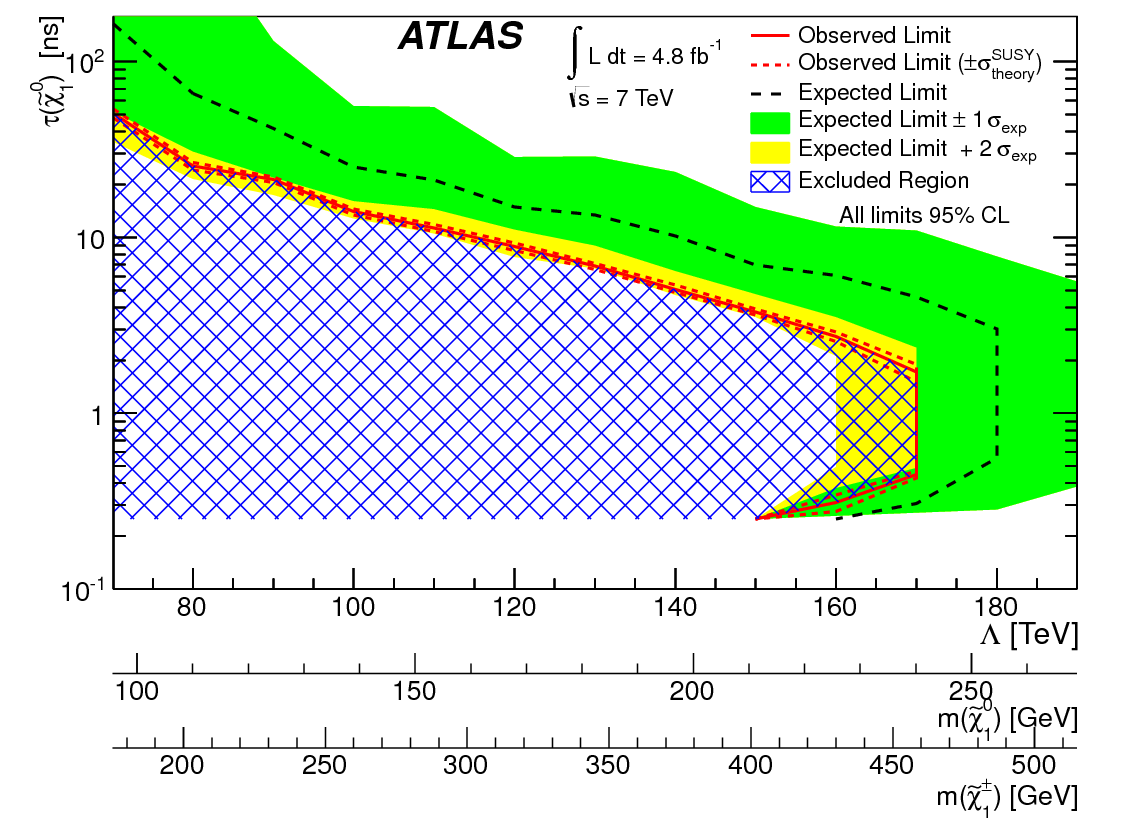
\includegraphics[height=3.0in,width=3.0in]
{THESISPLOTS/ATLAS_Upper_Limit.png} \quad
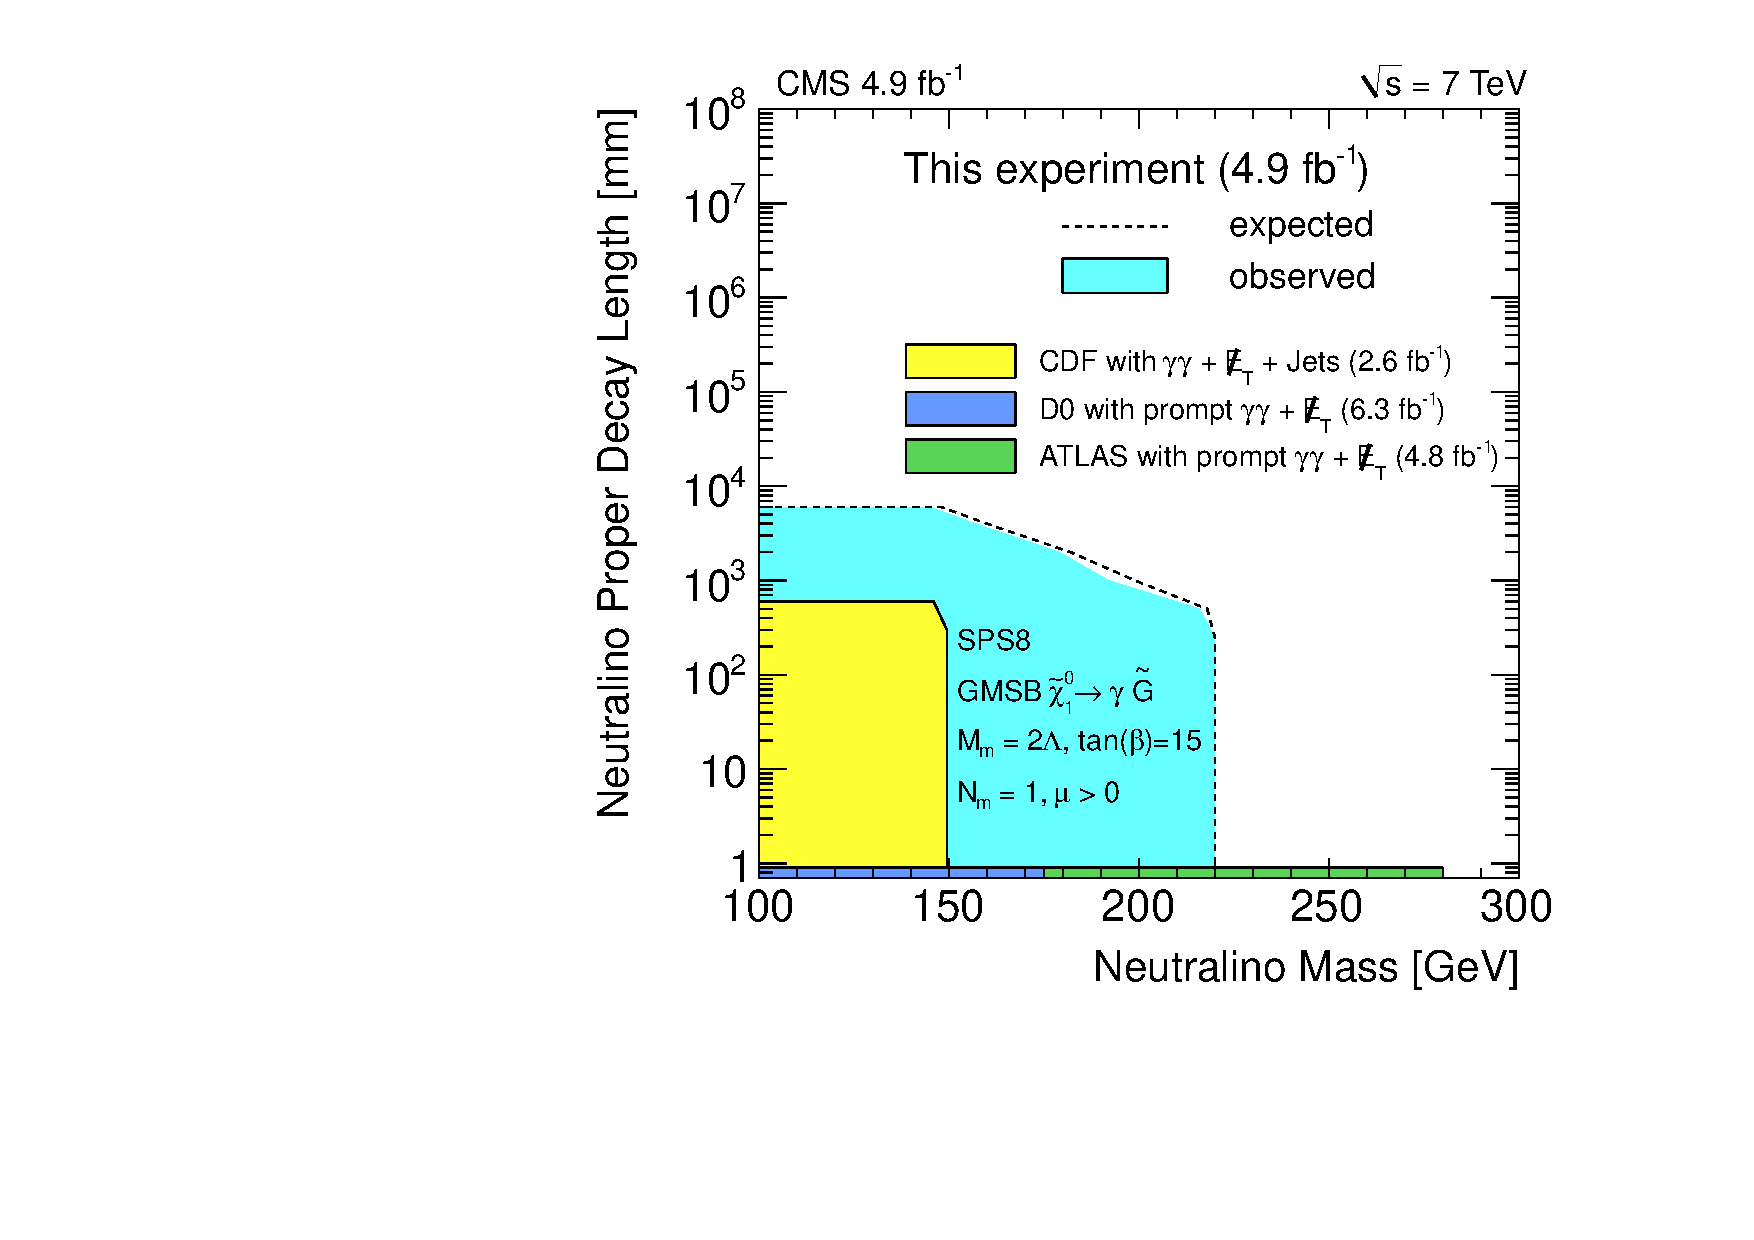
\includegraphics[height=3.1in,width=3.0in]{THESISPLOTS/2D_exclusion.pdf}}
\captionof{figure}{Neutralino lifetime and mass upper limit from ATLAS(left) and CMS(right) 7~TeV analysis with non-pointing photons and MET.}
\label{fig:UpperLimits}
\end{center}